%% ----------------------------------------------------------------
%% Thesis.tex -- MAIN FILE (the one that you compile with LaTeX)
%% ---------------------------------------------------------------- 

% Set up the document
\documentclass[a4paper, 11pt, oneside]{Thesis}  % Use the "Thesis" style, based on the ECS Thesis style by Steve Gunn
\graphicspath{Figures/}  % Location of the graphics files (set up for graphics to be in PDF format)
% Include any extra LaTeX packages required
\usepackage[square, numbers, comma, sort&compress]{natbib}  % Use the "Natbib" style for the references in the Bibliography
\usepackage{verbatim}  % Needed for the "comment" environment to make LaTeX comments
\usepackage{vector}  % Allows "\bvec{}" and "\buvec{}" for "blackboard" style bold vectors in maths
\hypersetup{urlcolor=blue, colorlinks=true}  % Colours hyperlinks in blue, but this can be distracting if there are many links.
%% ----------------------------------------------------------------

\begin{document}
% Set up the Title Page
\title  {Wi-Coverage: \\ An autonomous robot exploration coverage strategy using\\ \vspace{0.45em} Commodity WiFi}
\vspace{5em}
\authors  {\texorpdfstring
            {\href{vbehara@buffalo.edu}{Venkata Kali Suguna Praneeth Behara}}
            {Venkata Kali Suguna Praneeth Behara}
            }
\addresses  {\groupname\\\deptname\\\univname}  % Do not change this here, instead these must be set in the "Thesis.cls" file, please look through it instead
\date       {Feb 1, 2018}
\subject    {}
\keywords   {}
\maketitle
%% ----------------------------------------------------------------

\setstretch{1.3}  % It is better to have smaller font and larger line spacing than the other way round

% Define the page headers using the FancyHdr package and set up for one-sided printing
\fancyhead{}  % Clears all page headers and footers
\rhead{\thepage}  % Sets the right side header to show the page number
\lhead{}  % Clears the left side page header

\pagestyle{fancy}  % Finally, use the "fancy" page style to implement the FancyHdr headers

%% ----------------------------------------------------------------
% The "Funny Quote Page"
\pagestyle{empty}  % No headers or footers for the following pages
\null\vfill
% Now comes the "Funny Quote", written in italics
\begin{center}
\vspace{19em}
\textit{"Education is ones greatest asset" - My Mother}
\end{center}
%\begin{flushright}
%If the quote is taken from someone, their name goes here
%//\end{flushright}

\vfill\vfill\vfill\vfill\vfill\vfill\null
\newpage  % Funny Quote page ended, start a new page
%% ----------------------------------------------------------------
\frontmatter      % Begin Roman style (i, ii, iii, iv...) page numbering
\setcounter{page}{3}
% The Abstract Page
\addtotoc{Abstract}  % Add the "Abstract" page entry to the Contents
\abstract{
\addtocontents{toc}{\vspace{1em}}  % Add a gap in the Contents, for aesthetics

%The Thesis Abstract is written here (and usually kept to just this page). The page is kept centered vertically so can expand into the blank %space above the title too

Exploration of an apriori unknown environment by a mobile robot requires it to identify its next best position in the partially explored region which yields the maximum information. This thesis work will broadly answer two questions. Firstly, how can a robot perform an autonomous exploration if given a stereo vision and secondly given multiple such robots, how can they collaborate with minimal communication to efficiently explore an indoor environment using Wi-Fi as an additional sensor. 
To begin we describe the process of exploring frontiers which separate the explored from the uncharted regions, incorporating the method of maximizing the information gained for every frontier to be visited next. We then introduce a novel coverage strategy which combines the previous technique of frontier based exploration to using Wi-Fi signal strengths from surrounding access points. This approach involves clustering of environment without any prior information about it and demonstrate it to be complete i.e completely explore any given environment unlike most traditional coverage strategies which are either incomplete or probabilistically complete. Wi-Coverage was designed such that the robot explores in a systematic way and no prior access to the map is required. It also supports multiple robot coordination with minimum communication possible.

Robot Operating System (ROS) is used for implementation of frontier exploration and engineering issues faced are also discussed in detail. Gazebo simulator is used for simulating robots and Wi-Fi powered environments. Simulation results of time taken for full coverage and robot trajectories are obtained for the proposed strategy and are compared with best available form of frontier exploration which use optimal information gain policy.   
}

\newpage
%% ----------------------------------------------------------------
% Declaration Page required for the Thesis, your institution may give you a different text to place here
% \Declaration{

% \addtocontents{toc}{\vspace{1em}}  % Add a gap in the Contents, for aesthetics

% I, Venkata Behara, declare that this thesis titled, `Wi-Coverage : An autonomous exploration coverage strategy using Commodity WiFi' and the work presented in it are my own. I confirm that 

% \begin{itemize} 
% \item[\tiny{$\blacksquare$}] This work was done wholly or mainly while in candidature for a masters degree at this University.
 
% \item[\tiny{$\blacksquare$}] Where any part of this thesis has previously been submitted for a degree or any other qualification at this University or any other institution, this has been clearly stated.
 
% \item[\tiny{$\blacksquare$}] Where I have consulted the published work of others, this is always clearly attributed.
 
% \item[\tiny{$\blacksquare$}] Where I have quoted from the work of others, the source is always given. With the exception of such quotations, this thesis is entirely my own work.
 
% \item[\tiny{$\blacksquare$}] I have acknowledged all main sources of help.
 
% \item[\tiny{$\blacksquare$}] Where the thesis is based on work done by myself jointly with others, I have made clear exactly what was done by others and what I have contributed myself.
% \\
% \end{itemize}
 
 
% Signed:\\
% \rule[1em]{25em}{0.5pt}  % This prints a line for the signature
 
% Date:\\
% \rule[1em]{25em}{0.5pt}  % This prints a line to write the date
% }

% \newpage  % Declaration ended, now start a new page

\setstretch{1.3}  % Reset the line-spacing to 1.3 for body text (if it has changed)

% The Acknowledgements page, for thanking everyone
\acknowledgements{
\addtocontents{toc}{\vspace{1em}}  % Add a gap in the Contents, for aesthetics

I am very fortunate in having the support and encouragement of many people during my masters. First of all I would like to thank my co-advisor Karthik for giving me this opportunity and sharing his invaluable research insights and ideas. I also thank my co-advisor Nicholas Mastronarde for giving me valuable suggestions and academic support without which this work would not have been possible.

\hspace{1.5em} It has been hugely rewarding for being a part of Distributed Robotics and Networked Embedded Systems group: thanks everyone, past and present, for all the discussions, arguments and fun we had together! Each of you in your own way created a special place to work and learn. To Charu, I am grateful for his contributions, our research and for the countless interesting and stimulating conversations. I would also like to thank Zakieh for helping me with her technical expertise, whenever I needed it. Chen, Yifang made the lab a fun place to be and always provided intelligent inputs in the discussions.

\hspace{1.5em} Special thanks also go to my roommates, past and present, Kashyap Chitta, Sri Sadhan, Vamsi Eranki, Abhilash Gandla, Lokesh Boddu, Bodhi Rudra and Srinivas Addula for their encouragement and support, especially for the much needed dinner supplies.

\hspace{1.5em} Most of all, I am grateful to my family that always stood by me, helping me pursue my passion and guiding me to a better tomorrow.

}
\clearpage  % End of the Acknowledgements
%% ----------------------------------------------------------------

\pagestyle{fancy}  %The page style headers have been "empty" all this time, now use the "fancy" headers as defined before to bring them back


%% ----------------------------------------------------------------
\lhead{\emph{Contents}}  % Set the left side page header to "Contents"
\tableofcontents  % Write out the Table of Contents

%% ----------------------------------------------------------------
\lhead{\emph{List of Figures}}  % Set the left side page header to "List of Figures"
\listoffigures  % Write out the List of Figures

%% ----------------------------------------------------------------
% \lhead{\emph{List of Tables}}  % Set the left side page header to "List of Tables"
% \listoftables  % Write out the List of Tables

%% ----------------------------------------------------------------
\setstretch{1.5}  % Set the line spacing to 1.5, this makes the following tables easier to read
\clearpage  % Start a new page
\lhead{Abbreviations}  % Set the left side page header to "Abbreviations"
\listofsymbols{ll}  % Include a list of Abbreviations (a table of two columns)
{
\textbf{RSSI} & \textbf{R}eceived \textbf{S}ignal \textbf{S}trength \textbf{I}nformation \\
\textbf{LIDAR} & \textbf{LI}ght \textbf{D}etection \textbf{A}nd \textbf{R}anging \\
\textbf{Wi-Fi} & \textbf{Wi}reless \textbf{Fi}dility \\
\textbf{AP} & \textbf{A}ccess \textbf{P}oint \\
\textbf{SS} & \textbf{S}ignal \textbf{S}trength\\
\textbf{CSS} & \textbf{C}ustom \textbf{S}ignal \textbf{S}trength\\
\textbf{DoF} & \textbf{D}egrees \textbf{o}f \textbf{F}reedom\\
\textbf{ROS} & \textbf{Robotics} \textbf{O}perating \textbf{S}ystem\\
\textbf{ITU} & \textbf{I}nternational \textbf{T}elecommunication \textbf{U}nion\\
\textbf{RTAB} & \textbf{R}eal \textbf{T}ime \textbf{A}ppearance \textbf{B}ased\\
\textbf{RGB-D} & \textbf{R}ed \textbf{G}reen \textbf{B}lue - \textbf{D}epth\\
\textbf{UAV} & \textbf{U}nmanned \textbf{A}erial \textbf{V}ehicle
}

%% ----------------------------------------------------------------
% \clearpage  % Start a new page
% \lhead{\emph{Physical Constants}}  % Set the left side page header to "Physical Constants"
% \listofconstants{lrcl}  % Include a list of Physical Constants (a four column table)
% {
% % Constant Name & Symbol & = & Constant Value (with units) \\
% Speed of Light & $c$ & $=$ & $2.997\ 924\ 58\times10^{8}\ \mbox{ms}^{-\mbox{s}}$ (exact)\\

% }

%% ----------------------------------------------------------------
\newpage  %Start a new page
% \lhead{{Symbols}}  % Set the left side page header to "Symbols"
% \listofnomenclature{lll}  % Include a list of Symbols (a three column table)
% {
% % symbol & name & unit \\
% $a$ & distance & m \\
% $P$ & power & W (Js$^{-1}$) \\
% & & \\ % Gap to separate the Roman symbols from the Greek
% $\omega$ & angular frequency & rads$^{-1}$ \\
% }
%% ----------------------------------------------------------------
% End of the pre-able, contents and lists of things
% Begin the Dedication page

\setstretch{1.3}  % Return the line spacing back to 1.3

\pagestyle{empty}  % Page style needs to be empty for this page
\dedicatory{Dedicated to my loving family}

\addtocontents{toc}{\vspace{2em}}  % Add a gap in the Contents, for aesthetics


%% ----------------------------------------------------------------
\newpage
\mainmatter	  % Begin normal, numeric (1,2,3...) page numbering
\pagestyle{fancy}  % Return the page headers back to the "fancy" style
\lhead{\emph{Introduction}}
% Include the chapters of the thesis, as separate files
% Just uncomment the lines as you write the chapters

\chapter{Introduction}
\lhead{\emph{Introduction}}
Robots have been around us ever since the time of Leonardo da Vinci. The development in this field has seen a tremendous growth and intelligent robots are emerging in almost every field like automotive, medicine, defence which are just to name a few. We are in an era where intelligence has evolved from Shakey, the world's first intelligent robot to Sophia, the world's first robot who was awarded a citizenship.

\par Huge amount of research have been invested in robots to assist humans in tasks that are monotonous or dangerous. For example, the entry of autonomous machines such as Roomba\cite{1} not only revolutionized the industry of floor cleaning but also has brought robots much closer to humans which were instead confined in spaces around computer scientists. A bigger example is the recent bloom of autonomous cars. Almost all automotive as well as software companies have their dedicated R\&D for self-driving cars and numerous technologies are being developed and tested every day. These autonomous robots not only make our lives easier but also play a crucial role in applications of autonomous exploration such as search and rescue, mine detection, etc. 

\par Autonomous robots are intelligent machines capable of performing tasks in the world by themselves, without explicit human control. These intelligent machines must posses and exhibit the following qualities\cite{6}
\begin{itemize}
    \item Avoid harmful situations especially to humans, itself and fellow robots, unless its designed to do so. 
    \item Work for an extended period of time without any human intervention.
    \item Gain information about the environment by sensing it.
\end{itemize}
This work is about autonomous exploration of a-priori unknown environments with mobile robots. Hence forth all discussions are focused on autonomous mobile robots unless specified.

\section{Autonomous robots}
While many robots can navigate using maps, few can build their own maps. Mobile robots need a map to effectively navigate in their environment. The ability of mobile robots to autonomously move in an unknown environment to gather the sensory information required to build a map for navigation is called autonomous exploration. A good exploration strategy is one that generates a complete or nearly complete map in a reasonable amount of time. Exploration and map-building are extensively researched by robotics community due to its wide range of real-world applications. Such applications may include search and rescue, hazardous material handling, military actions, planetary exploration, path planning, and devastated area exploration\cite{17}. Generally, autonomous robot is able to incrementally construct a model (map) for its environment based on the sensory information gathered in an online fashion, i.e. while navigating through the environment. This process requires choosing the best next location for the robot to visit, planning the shortest path to reach that location and finally controlling the robot’s motion in its journey to that location. 
\par Autonomous mobile robots interact with their environment to get an internal representation of the environment. For any autonomous mobile robot to explore or cover an unknown environment, the following are the prerequisites, 
\begin{itemize}
    \item Accurately map the environment and simultaneously get a position estimate of itself in the mapped environment.
    \item Navigate itself through environment which might be dynamic as well.
    \item Increase its extent of the partially explored map and completely explore the environment.
\end{itemize}

\par Simultaneous localization and mapping technique is often used to construct a map for the environment and localize the robots in it. As the robots move to unexplored new areas, these areas are then included in the map. But there are a number of questions to be answered in designing an autonomous exploration strategy. The key challenges in autonomous exploration are

\begin{itemize}
    \item How does the robot extend its partially explored map?
    \item How a robot plans in order to visit the remaining unexplored areas while minimizing the total traveled distance?
    \item In case of multiple robots, how do they distribute the unexplored space efficiently?
\end{itemize}

\section{Motivation}
If a robot is equipped with a vision sensor, where should it move after it is switched on? In this work we answer this question by using a frontier based exploration approach wherein the bot attempts to look at, thus map every boundary which separates the reachable space from the uncharted, known as the frontiers. Ideally the bot has to move to these boundaries to expand its map. Given, the robot explores the frontiers it senses, which frontier is to be selected as its next position in the environment such that the exploration is efficient? Using Wi-Fi how is the robot motion planned such that it covers the entire environment? How do multiple such robots distribute the environment and efficiently explore with minimum communication possible? All the above questions posed form the key motivation for Wi-Coverage. Through this work, we would like to introduce Wi-Fi as a readily available ubiquitous sensor to help assist explorations or perform search operations in huge places like airports, mall, etc.
\par An additional motivation for Wi-Coverage are Robot operating system (ROS) and Gazebo. ROS is an open source software framework available which makes a roboticist's life better by providing low level drivers and interface with physical parts of the robot. Gazebo developed by Willowgarage is a simulation platform capable of simulating life like real world scenarios much better than the older platforms like Stage. Several coverage algorithms are devised using ROS, but only few of them are directed towards online mapping and multi robot explorations, and on the idea of simulating using Gazebo. 

\section{Frontier Exploration}
Given the ability to sense the environment around it, when a mobile robot is switched on, how does it know where to go next which increases the extent of its map? Well, a simple approach would be to make the robot move in a pattern, for example in concentric circles\cite{9}. Though this approach would extend the horizons of the map, it would not guarantee that we completely explore the environment. A much clever method would be to reach an empty space in the partially explored environment. For example, imagine a scenario where we enter a new apartment. In an attempt to explore the new environment, we move to the boundaries up to where we are able to see and are reachable. We finally explore the whole place like rooms and porch by repeating the same until there is no such boundary left.  Exploration can be described as the act of moving through an unknown environment while building a map that can be used for subsequent navigation\cite{10}. This approach is popularly known as the frontier based exploration which we used in this work.

\par Exploring frontiers will eventually complete visiting every place in the environment. The way in which the frontiers are explored, decides the effectiveness of the algorithm. In other words, which frontier to pick next such that the robot completes the entire space in the least amount of time? This is our next challenge. A popular solution is to maximize the information gain at every frontier such that the new information about the environment obtained at every position the robot visits is maximum in the current map. Though this approach is efficient, the bots path is highly unpredictable and depends on the sensors precision and sensitivity. In this work we propose a variant to this approach by using Wi-Fi sensing i.e sensing the signal strength from various Wi-Fi routers to aid the bot in exploring the environment in a more systematic way. In addition to using the information gain formulation ,we associate the RSSI from the surrounding Wi-Fi routers to it. This helps the bot cluster the environment and explore it systematically. This approach does not require any prior information about the environment i.e all processes are performed online. This novel approach particularly has an edge over traditional methods in terms of communication between robots in collaborative robotics.

\section{Wi-Fi as an additional sensor} 

Very often, it is evident that using multiple sensors outperform the efficiency, when instead used a single sensor. Additional information is either fused with the primary information or directly used in consequent stages to increase accuracy and performance of the policy. In some cases, augmenting with additional data can help overcome the limitations of the actual sensor. Wi-Fi routers have become ubiquitous for quick internet access in most urban settings including offices, homes, and public spaces such as malls and airports. Most robots are typically equipped with a Wi-Fi radio for communication as well. Our conjecture was that we could use Wi-Fi as an additional sensing modality which can provide improved solutions when augmented with the primary sensor(s) information. In this work, we demonstrate how the policy of picking frontiers can be improved in case of frontier exploration such that the robots path is systematic and predictable. We show that by using this additional sensor we can overcome the range limitation of a stereo camera and understand the environment in a much greater sense.

% \section{goals}

% % Two of the significant branches in the robotics are autonomous robot exploration and cooperative robotics. Autonomous robot exploration involves robot exploring a space without any human interaction or assistance. They are differentiated from remote controlled, or tele-operated mobile robots in the fact that there is no human in the loop controlling a robots movement. In other words, the robots decision and executes of its choices are all computerized\cite{25}.
% The areas of robotic research in the second half of twentieth century have covered a breadth of topics including human-assisting robots, home automation robots, industrial manufacturing robots, search and rescue robots and many more. Two of the significant branches in robotics are autonomous robot exploration and cooperative robotics to which we would like to contribute. There are two main goals in this thesis. The first one is to use vision and inexpensive off the shelf components and implement a frontier based exploration available in its best form which is by maximizing information gain. The other one is to develop an online policy for exploring an unknown environment using commodity WiFi which extremely minimizes the communication efforts between robots in a cooperative environment while almost maintaining the maximum coverage and time possible by efficient exploration techniques like frontier based exploration using information gain. As a part of this we will see on how to use commodity Wifi as an additional sensor which is very much an abundant and useful resource found in every indoor space, to aid the main sensors solving the coverage problem in a much more systematic way.  

\section{Thesis organization}    
We begin, in Chapter 2, with an overview of research done in the field of exploration and numerous coverage strategies. Chapter 3 describe our implementation of frontier based exploration using a vision sensor and ROS. We then describe our novel coverage strategy, Wi-Coverage in both single and multi robot scenarios. The pipeline and design of frontier selection using Wi-Coverage is described in detail. Later in the chapter, we present some engineering issues faced in implementing the frontier based exploration and methods to solve them. 
A robot is a conglomeration of complex software and hardware components. Chapter 3 also describes the robot, Darwin used in this work and at DRONES Lab. We present the software ROS: its essential components and protocols, which we used in this work and its high level packages like RTAB-Map and move base. Experiments and results are presented in Chapter 5. Chapter 6 contains concluding remarks and an outline of future work. 

\section{Contributions}
The main contributions of this thesis are as follows:
\begin{itemize}
    \item An implementation of frontier based exploration using vision and solving the engineering problems faced while realizing it in the real world.
    \item A coverage strategy which uses a freely available resource, Wi-Fi, to assist the robot(s) in exploration of unknown environment. This strategy also considerably minimizes the communication required between robots in a multi robot scenario.
    \item Design of simulation environments with software configurable Wi-Fi routers with multiple signal strength models in Gazebo simulator.
\end{itemize} % Introduction

\chapter{Background}
\lhead{\emph{Background}}
This chapter presents an overview of topics which are either prerequisites for autonomous exploration and coverage behaviour presented in the later chapters, or provide alternative solutions to the questions we are uncovering of how a robot can choose to move and coordinate.

\section{Overview}
Autonomous robots are systems which sense, actuate, compute and communicate. Sensing can be an ability to see, feel, hear or even a combination of them. For example a bot with a Kinect sensor has the ability to see. Similarly a bump sensor or a laser scanner attached to a bot will power it up with the ability to feel the presence of the obstacles around it. Actuation in this case is the bots' ability to move in the world. the following are the important functions and capabilities an autonomous robot 
must possess over other types of robots as summarized in \cite{7},
\begin{itemize}
    \item Gain information about the operating environment.
    \item Work for an extended period of time without human intervention.
    \item Move itself throughout its operating environment without human assistance.
    \item Avoid situations that are harmful to people, property, or itself unless those are designed so.
\end{itemize}
\vspace{5em}
This chapter will cover the following topics,
% \par Pose estimation : What is the sensors position with respect to a global reference frame, and how is it updated with the motion model? The SLAM problem.

\par \textbf{Mapping} : The robot plans its motion and performs exploration using a global map. Given a pose estimate and sensor data at the position, how do we integrate it into a globally consistent map structure?

\par \textbf{Exploration} : The robot should extend its global frame such that it covers the entire given space. Given a map and a current pose, how do we take high level decisions like where should the robot move next to achieve the above? 

% \par \textbf{Motion planning}: How is the robot made to move across the environment expanding the horizons avoiding fixed and dynamic obstacles?

% \section{Pose estimation}
% Assuming the robot has an initial scan of its immediate environment, we need to locate the robot with respect to its initial pose. It has to maintain an internal estimate of its position and orientation in the world. The pose estimate for a robot confined to ground plane will have two transnational components and one rotational component,
% \begin{equation} 
%     \textbf{p} = [x,y,z, \theta_{r},\theta_p,\theta_y]^T
% \end{equation}
% where $\theta_{r}, \theta_{p}, \theta_{y}$ are the roll angle around the x-axis, pitch angle around the y-axis and yaw angle around the z-axis. These six degrees of freedom are often referred to as 6DoF. The following are some standard methods for such estimate.

% \subsection{Dead reckoning}
% In navigation, dead reckoning is the process of calculating one's current position by using a previously determined position, or fix, and advancing that position based upon known or estimated speeds over elapsed time and course\cite{19}. 

% \subsection{Laser scan matching}

% \subsection{Visual odometry}

\section{Mapping}
Mapping is one of the core competencies of truly autonomous robots\cite{25}. Acquiring maps with mobile robots can be challenging for a number of reasons according to \cite{25}. First, even under discrete approximations, such as grid approximation, maps can be described in $10^5$ or more variable, making it challenging to calculate the full posteriors considering such high dimensional space. Second, As the robot moves through the environment, it accumulates errors in odometry, making it gradually less certain of its location in the map. Having this localization challenge, mapping also gradually becomes tough, since the robot's position becomes uncertain - The SLAM problem.

\subsection{Map representations}
To express the process of generating measurements, we need to specify the environment in which a measurement is generated. A map of the environment is a list of objects in the environment and their locations. While a topological map is concerned with the connections between locations and stored in a graph-like structure, a metric map maintains a model of the environment in a geometric sense which corresponds more directly to the real world. We used an occupancy grid as our map representation since frontier exploration works well with a grid based mapping approaches. The following are some representations of metric maps.

\subsubsection{Point clouds}
Point cloud representation is one of the closest forms of representation to the actual surroundings. The range sensor detects points in space and are then transformed into a global coordinate frame. These are then added to an existing collection which forms the point cloud. An example of a point cloud is shown above in Fig. 2.1.  

\begin{figure*}
    \begin{subfigure}[b]{0.498\textwidth}
		\centering
		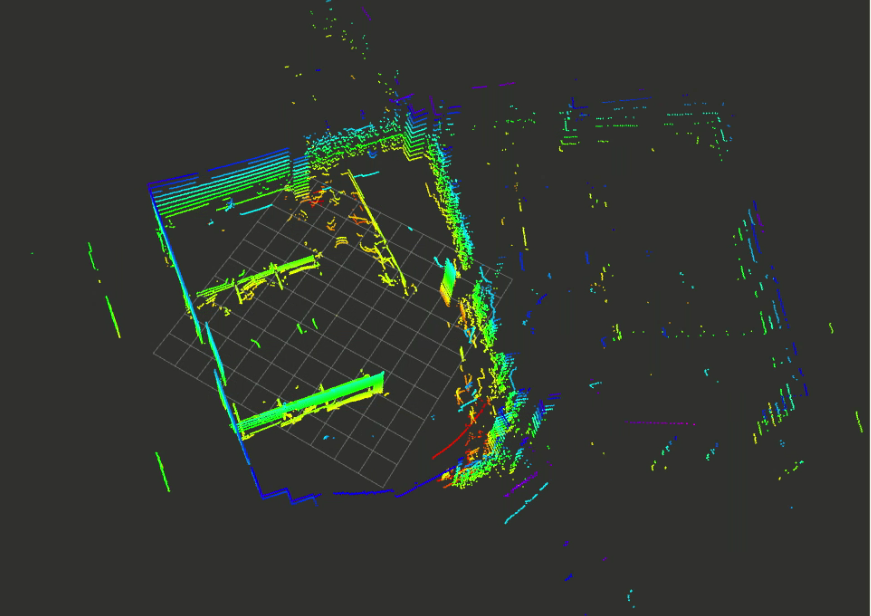
\includegraphics[width=\textwidth]{images/Symmetry_ppt.png}
		\label{subfig:a}
		\caption{}
		\vspace{2em}
	\end{subfigure}
	\begin{subfigure}[b]{0.498\textwidth}
	    \centering
		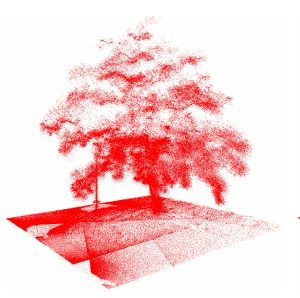
\includegraphics[width=\textwidth]{images/occupancytree.png}
		\label{subfig:b}
		\caption{}
	\end{subfigure}
    \caption{From left to right: Point cloud map representation using a VLP-16 LIDAR of the Drones Lab. A point cloud of a tree. Image from \cite{21}}
\end{figure*}

\subsubsection{Occupancy grids}
A classical map representation is known as occupancy grid map. Occupancy maps are location-based: They assign to each x-y coordinate a binary occupancy value which specifies whether or not a location is occupied with an object. Occupancy grid maps are great for mobile robot navigation\cite{25}. In other words, they make it easy to find paths through the unoccupied space. An occupancy grid is a quantified workspace with evenly spaced volumetric elements called voxels. Each voxel stores a probability of occupancy, i.e an estimate of whether there is an obstacle in that grid space. These probabilities are thresholded resulting in three values: \\
\noindent \textbf{Free} - This voxel or grid has been explored and is free of obstacles.\\
\textbf{Occupied} - This space has obstacles and robot senses that it cannot move into that space.\\
\textbf{Unknown} - The uncharted space that the robot needs to explore and get an idea of its occupancy.

\par These values can be represented using any random numbers but only that the nomenclature is to be persistent. The boundary upto which the robot can see or sense is called the horizon and the boundary which separates the free space with the unknown space is called the frontier. Each such cell which form the boundary is called a frontier cell. 

As per \cite{12}, the gold standard of an occupancy grid algorithm is to compute its posterior over the maps given data according to equation 2.1

\begin{equation} \label{eq:posterior}
    p(m|z_{1:t},x_{1:t})
\end{equation}

\noindent where \textit{m} is the map ${z_{1:t}}$ are the set of measurements up to time \textit{t}, and ${x_{1:t}}$ is the robot path, i.e the sequence of all its poses. ${m_i}$ refer to the index in each cell \textit{i}. Throughout this work $p(m_i = 100)$ is the probability that cell $m_i$ is occupied, and conversely $p(m_i = 0)$ is the probability it is empty. If $p(m_i = -1)$, it refers to the grid cell being an unknown cell. The posterior map probability given the sensor and the motion model is the product of the posteriors of each grid cell which is given by equation 2.2. 

% \begin{equation}
%     p(m|z_{1:t},x_{1:t})
% \end{equation}

% \noindent where $z_{1:t}$ is the set of all measurements until current time \textit{t}, and $x_{1:t}$ is the corresponding set of robot poses. the posterior of a map over the entire map can be given as the product of each grid cell,

\begin{equation}
    p(m|z_{1:t},x_{1:t}) = \prod_i{p(m_i|z_{1:t},x_{1:t})}
\end{equation}

Not only that occupancy grids are easy to construct and maintain, they work well in dynamic environments. Fig 2.2 represents an occupancy grid corresponding to the blue print of the environment which is inaccurate in certain places\cite{25}. If some data is corrupted by the presence of people; the occupancy grid map filters it out quite nicely. This makes occupancy grid maps much better suited for robot navigation than sets of scan endpoint data.

\begin{figure*}
    \begin{subfigure}[b]{0.498\textwidth}
		\centering
		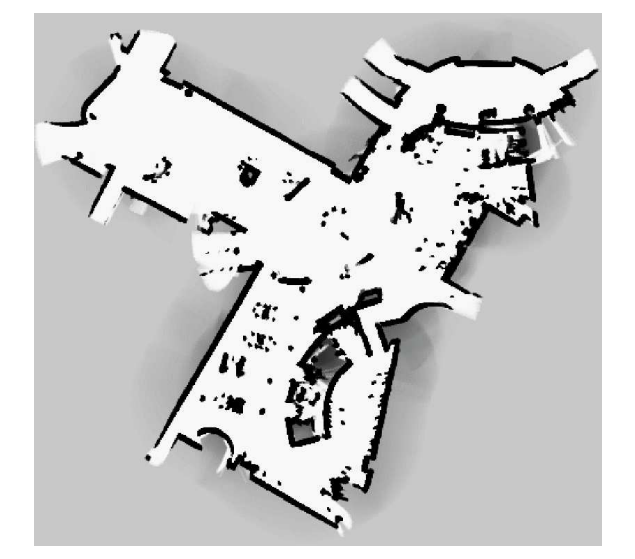
\includegraphics[width=\textwidth, height=0.75\textwidth]{images/occ1.png}
		\label{subfig:a}
		\caption{}
		\vspace{2em}
	\end{subfigure}
	\begin{subfigure}[b]{0.498\textwidth}
	    \centering
		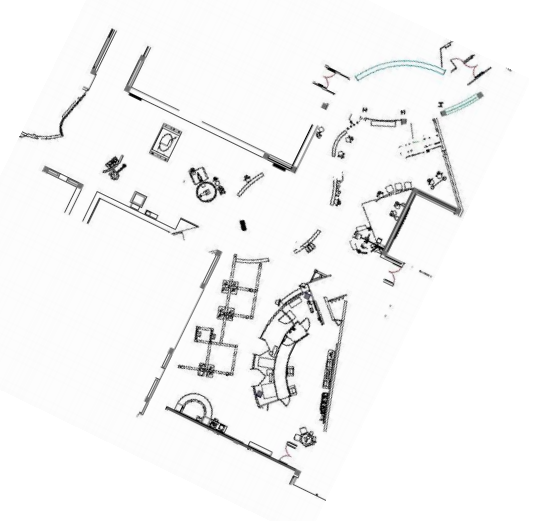
\includegraphics[width=\textwidth, height=0.75\textwidth]{images/occ2.png}
		\label{subfig:b}
		\caption{}
	\end{subfigure}
    \caption{(A)Occupancy grid map and (B)architectural blue-print of a large open exhibit space. Image from \cite{25}}
\end{figure*}

\subsubsection{2.5D Maps}
Handling full 3D occupancy grids can be challenging especially in can of limited computational resources. These limitations can be ameliorated when dealing with a robot constrained to the ground plane. 2.5D or elevation maps are a better alternatives to full 3D maps in such situations. These cells contain an estimate of the surface height at that position and can be sufficient for navigation and exploration\cite{12}\cite{13}. An example of a 2.5D map can be seen in Fig 2.3 above. The disadvantage of these map structures is that they are limited to a single height value at each cell, meaning environments containing multiple levels such as bridges or underpasses cannot be represented. Another disadvantage is their inability to represent free-space or unexplored regions numerically\cite{11}.  

\begin{figure}
    \centering
    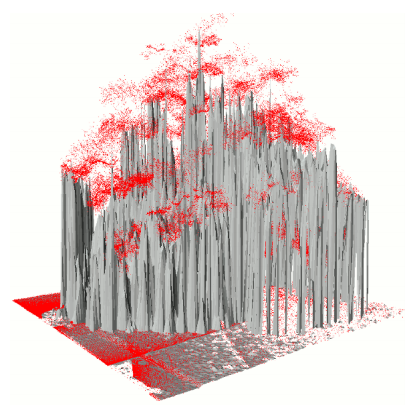
\includegraphics[width=0.5\textwidth]{images/25D.png}
    \caption{A 2.5D map of a tree. Image from \cite{21}}
    \label{fig:my_label}
\end{figure}

% % \section{Localization}
% \subsection{SLAM}
% \subsection{Path Planning}

\section{Autonomous Exploration and Coverage}
Exploration can be defined as maximizing the knowledge about the external world or simply the surroundings. Exploration has been a paramount problem in the field of robotics. A number of instances can be listed where exploration can help achieve a particular purpose like floor cleaning, detecting mines in an abandoned mine site, identifying humans stuck in disaster effected sites\cite{9}, interstellar explorations\cite{10}, etc. This in general, require the robotic device to be able to navigate. 
Autonomous exploration is a derivative of Coverage problem. Coverage simply implies the exploration performed has to cover the entire environment. Depending on the sensor(s) used, there are several applications like floor cleaning, lawn mowing, mine sweeping, search and rescue, etc. Exploration algorithm itself might not be complete and requires a coverage strategy to make it complete. Coverage is analogous to covering salesman problem, a variant of traveling salesman problem where the agent has to travel the neighborhood of the city as opposed to just visiting the city as in traveling salesman problem\cite{28}. 

\subsection{Traditional Coverage Approaches}

\begin{figure*}
    \begin{subfigure}[b]{0.498\textwidth}
		\centering
		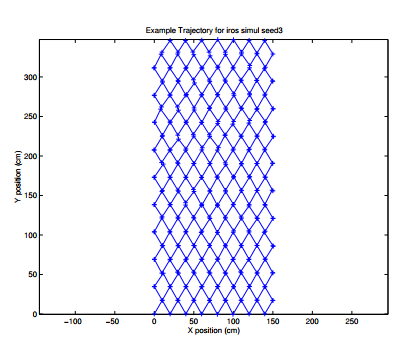
\includegraphics[width=0.85\textwidth, height=0.85\textwidth]{images/seed.png}
		\label{subfig:a}
		\caption{}
	\end{subfigure}
	\begin{subfigure}[b]{0.498\textwidth}
	    \centering
		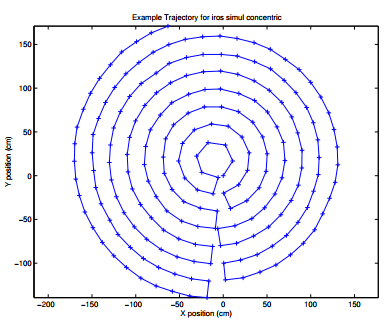
\includegraphics[width=0.85\textwidth, height=0.85\textwidth]{images/conc.png}
		\label{subfig:b}
		\caption{}
	\end{subfigure}
	\begin{subfigure}[b]{0.498\textwidth}
	    \centering
		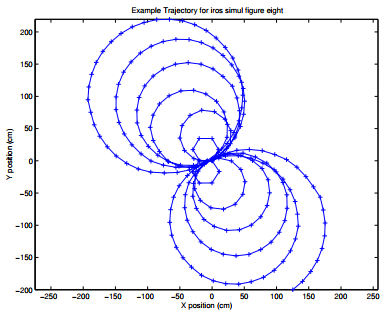
\includegraphics[width=0.85\textwidth, height=0.85\textwidth]{images/eight.png}
		\label{subfig:c}
		\caption{}
	\end{subfigure}
	\begin{subfigure}[b]{0.498\textwidth}
	    \centering
		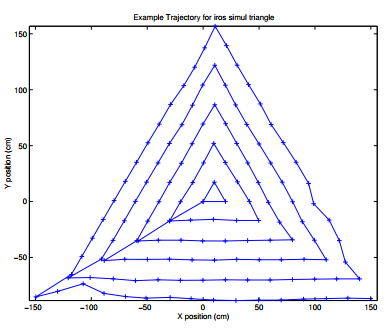
\includegraphics[width=0.85\textwidth, height=0.85\textwidth]{images/triangle.png}
		\label{subfig:d}
		\caption{}
	\end{subfigure}
	\begin{subfigure}[b]{0.498\textwidth}
	    \centering
		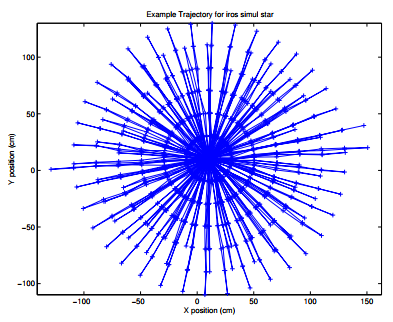
\includegraphics[width=0.85\textwidth, height=0.85\textwidth]{images/star.png}
		\label{subfig:e}
		\caption{}
	\end{subfigure}
    \caption{Different systematic approaches. Image from \cite{13}}
\end{figure*}

The early works in autonomous coverage can be classified into systematic or heuristic approaches and Non systematic approaches. Most of them suffer with atleast one drawback which includes incompleteness i.e they do not guarantee a successful exploration of the complete environment or they are probabilistically complete.

\textbf{Systematic approaches}: These approaches make the robot move in pre-defined patterns such that it unlocks new poses in the environment thereby exploring it.

\textbf{Non Systematic Approaches}: These approaches either rely on a random number generator or classify spaces to identify free space and usually involve a start-goal scenario.

\subsection{Systematic Approaches}
These are a set of heuristic behaviours that robots exhibit such as going in concentric circles, following a wall or evading obstacles\cite{8}. A combination of such behaviors can make the robot capable of accomplishing complex tasks like exploration. A variety of exploration trajectories have been developed and tested both in terms of coverage time as well as robot localization while executing the heuristic behavior. Some of them are described below\cite{26},

\noindent \textbf{Seed Spreader}: The robot follows a seed-spreader pattern through the environment\cite{27} as shown in Fig 2.4 (A).\\
\noindent \textbf{Concentric Circles}: The robot from its starting point goes in concentric circles reversing the direction for alternating circles as shown in Fig 2.4 (B).\\ 
\noindent\textbf{Figure Eight}: Similar to concentric circles, the robot traces them in a series of growing figure-eights, bringing the robot close to its starting point with each pass like shown in Fig 2.4 (C).\\ \noindent \textbf{Triangle}: The robot traces concentric equilateral triangular patterns shown in Fig 2.4 (D).\\ 
\noindent \textbf{Star}: This pattern makes the robot visit the starting point at each pass. The robot projects itself linearly and retraces the route only repeating it with a uniform difference in orientation at each pass. Fig 2.4 (E) shows the star pattern.\\

All the above strategies are proven to be either incomplete or probabilistically complete. The graph shown in Fig 2.5 shows the exploration efficiency plotted based on the images\/time step\cite{26}.

\begin{figure}
    \centering
    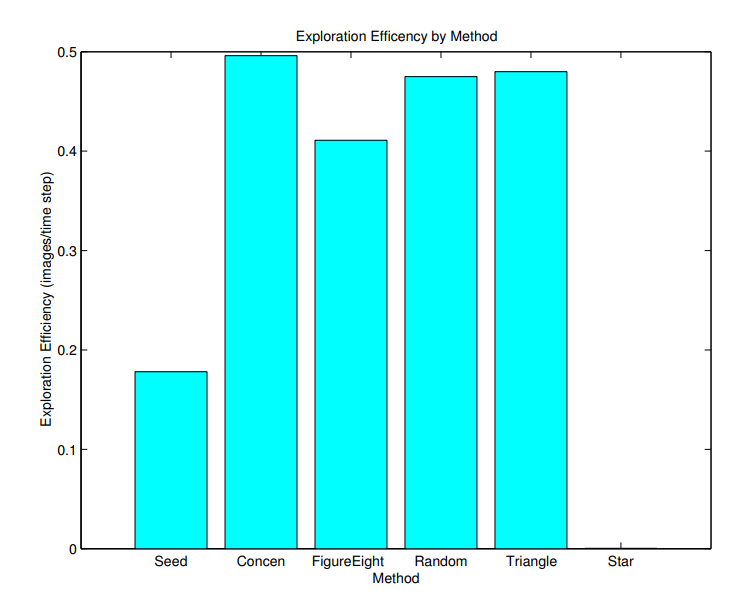
\includegraphics[width=0.75\textwidth]{images/expoeff.png}
    \caption{Evaluation of heuristic approaches discussed in Section 2.3.2}
    \label{fig:my_label}
\end{figure}

\subsection{Non Systematic Approaches}
These approaches do not follow a particular pattern or a heuristic and the trajectories covered are mostly unpredictable. The robot follows a formulation in order to pick its next move. The following are some non systematic approaches described.

\subsubsection{Random Approaches}
In this approach the robot selects a random pose with a threshold distance from itself. If it is unoccupied, the robot moves to it and repeats the same. This method have the following drawbacks,
\begin{itemize}
    \item The robot might end up picking already explored areas rendering the approach inefficient.
    \item Assuming the robot would pick all available poses in the environment, this approach is probabilistically complete.
\end{itemize}
A little smarter version is to select locations which are not explored. This would guarantee that the environment would be completely explored and hence makes the approach a complete one. These approaches are advantageous in terms of computational resources required but still prove to be inefficient in most cases when compared to other approaches such as frontier exploration.

\subsubsection{Frontier exploration}
A number of algorithms have being proposed for autonomous explorations. Frontier based exploration is one old and naive technique which is proved complete. This algorithm frees the robot to explore unknown spaces without the knowledge of prior data of obstacles in the given space. Frontier based exploration usually operate on grid maps. Unlike in other geometrical feature detection based maps like point or line maps, these maps distinguish between free, previously unexplored regions as shown in the Fig 2.6. The idea of frontier based exploration strategies is to guide the robot to the frontiers or boundaries between cells known to be free and cells for which no information is available\cite{25}. 

\begin{figure}
    \centering
    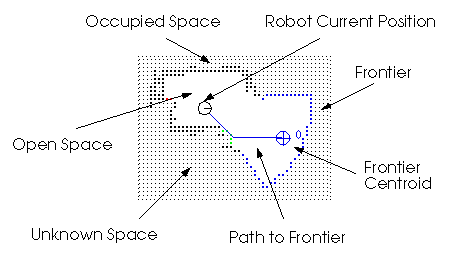
\includegraphics[width=0.75\textwidth]{images/frontier1.png}
    \caption{Imaging representing types of cells classified on an occupancy grid for frontier exploration}
    \label{fig:my_label}
\end{figure}

\subsection{Information gain exploration}
The above problem can be reduced to finding the next frontier which is logically considered to be the closest. This implies that the amount of information assigned or acquired at any frontier is the same. A better approach in finding the next poses which maximize expected uncertainty reduction. We implemented this approach for the comparative results in Chapter 4. 

\subsubsection{Entropy}
In information theory the measure of the information in a probability distribution \textit{p(x)} is the entropy \textit{$H_p(x)$} and is given by
\begin{equation}
    H_p(x) = - p(x)logp(x)dx
\end{equation}
Entropy is the measure of uncertainty associated with a random variable. $H_p(x)$ is maximal for a uniform distribution and this intuitively means that uncertainty is highest when all outcomes are equally likely. $H_p(x)$ decreases when $p(x)$ peaks and reaches zero when the outcome of the random trial is certain.

\subsubsection{Information gain}
The decrease in entropy between successive measurements is defined as the information gain \textit{I}. In the context of exploration this means that the difference in entropy at \textit{t+1} and at \textit{t} measures the information gained. Mathematically \textit{I} for a single voxel\/cell in an occupancy grid can be given by
\begin{equation}
    I(m_i|z_i) = H(p(m_i)) - H(p'(m_i|z_t))
\end{equation}
where, $p'(m_i|z_t)$ is the updated probability for the cell $m_i$ after updating the cell with a new measurement $z_i$ through the sensor model. The inverse sensor model allows us to estimate the information gain which we could expect if we were to move to a hypothetical new pose. This can be possible by ray-tracing through the occupancy grid, tracking the cells through which the ray passes. We follow a simple yet efficient method to measure the information gain by counting the number of unknown cells around each given frontier cell in a considerable radius.

\subsection{Cellular Decomposition}
These methods are developed to overcome the drawbacks of the above discussed approaches which are incomplete or probabilistically complete. All coverage approaches these days, that provide provable guarantee of completeness, use cellular decomposition\cite{35}. Three major classifications of cellular decomposition are approximate cellular decomposition which work on grid based representation of the free space, semi-approximate cellular decomposition which partially discretize the space and exact cellular decomposition is dividing the space into non intersecting regions.

\subsubsection{Approximate cellular decomposition}
This is a fine-grid representation where the union of all the cells only approximates the environment\cite{35}. In general, each cell in the grid is the size of robot's footprint which implies the cell is covered if the robot visits it. Complete coverage is achieved when all cells in the decomposition are visited. Zelinsky et al\cite{36} used conventional wavefront algorithm to achieve complete coverage. The wavefront algorithm initially assigns 0 to the goal, 1 to all of its neighbours and the remaining unmarked cells are labeled with a 2. This process is continued until the wavefront crosses the start and the robot uses a gradient descent on this numeric potential function\cite{37} to find a path.

\subsubsection{Semi-Approximate cellular decomposition}
Hert and Lumelsky developed a coverage algorithm that relies in a partial discretization of space where cells are fixed in width but the floor can have any shape\cite{38}\cite{39}. The robot can start at an arbitrary location in the map and perform zigzags along parallel straight lines. The smaller uncovered areas called inlets are detected by the robot and covered immediately in a depth-first order. The algorithm requires that the robot remember points at which it enters and exits inlets it covers assuring that each inlet is covered only once. 

\begin{figure}
    \centering
    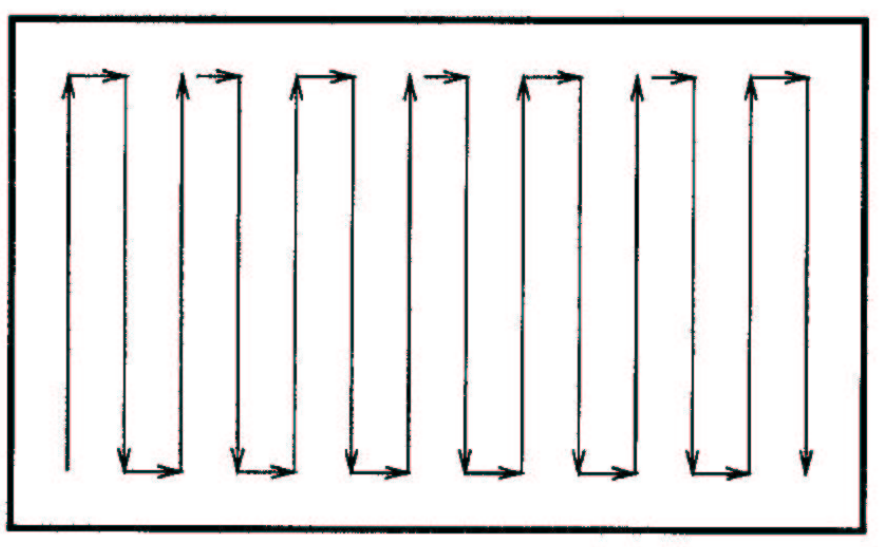
\includegraphics[width=0.5\textwidth]{images/bostrephroden.png}
    \caption{lawn mower trajectory: back and forth motions}
    \label{fig:my_label}
\end{figure}

\subsubsection{Exact cellular decomposition}
An exact cellular decomposition is the set of non-intersecting regions called cells, whose union fills the target environment\cite{35}. The robot can cover each cell using simple back-and-forth motions, reducing the coverage problem to motion planning problem.
Trapezoidal decomposition\cite{40} is a popular example of exact cellular decomposition technique where the free space is decomposed into trapezoidal cells. Each such cell is covered with simple back and forth motion shown in Fig 2.7. Coverage is achieved by visiting each cell in the adjacency graph. 
Boustrophedon decomposition is an extension to trapezoidal decomposition where many such trapezoidal cells can be merged such that no obstacle is in the robots path. Choset and Pignon\cite{35} developed this technique wherein new cells are added of the back-and-forth motion is obstructed by an obstacle and if not two cells are merged back into one cell as shown in Fig 2.8. 

\par All of the above techniques are proven to complete and neither of them require aprior information about the map. The weakness of these techniques would be their dependence on the grid resolution of the world. In order to perform complete coverage online, most techniques requires the robot to store information about the partially explored environment and perform additional computation to avoid edge cases such as revisiting a covered space. The disadvantage is that the complexity scales with the environment.  
% \subsubsection{Potential fields}
% \subsubsection{Graph methods}

\begin{figure}
    \centering
    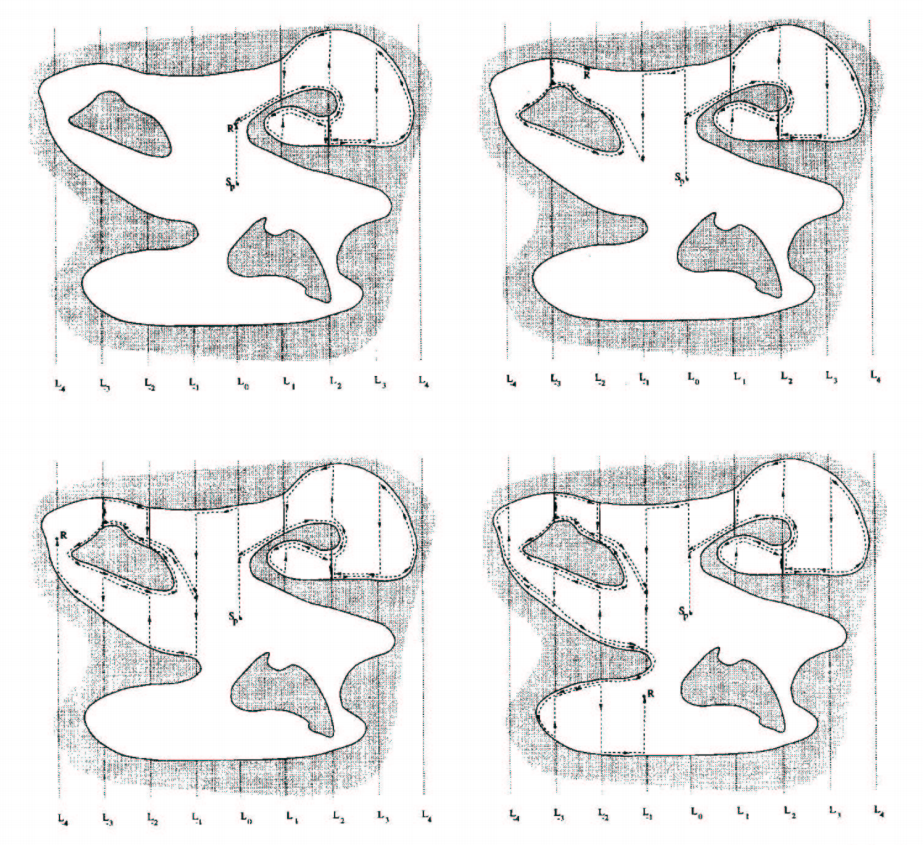
\includegraphics[width=\textwidth]{images/semiapproximate.png}
    \caption{A robot path using semi-approximate cellular decomposition in a map with islands and inlets. Images from \cite{35}}
    \label{fig:my_label}
\end{figure}

\section{Multi-Robot Coverage}
To reap the benefit of scaling efficiency with number of robots, multi robot exploration has been extensively researched in robotics community. The primary idea of using multiple robots is to improve coverage time. Though using multiple robots is advantageous, it does come with a set of challenge. The following are the prerequisites:
\begin{itemize}
    \item Communication network between robots for coordination
    \item Path planning utilities for robots
    \item Coordination schemes: Centralized or distributed
    \item Coverage strategy
\end{itemize}

\subsection{Coordination Control}
Typically two schemes for coordination between robots are available:

\noindent \textbf{Centralized Coordination scheme}:
Using a central coordinator, generally one of the robots or a separate system is deployed to help communication possible between robots. This master robot or system assigns the navigation tasks to the robots and make sure all the components are working properly. The benefit of using such a scheme is that its easier to implement but has a probability of single point failure. In other words, if the central node fails, the entire system crashes.

\noindent \textbf{Decentralized or distributed control}:
As the name indicates, in this scheme the robots are self reliant and take their own navigation decisions. These robots are connected using a Wi-Fi network and communicate their respective positions and progress. Though this scheme does not suffer from single point failure, the communication traffic in the network plays a role in deciding the algorithms efficiency.

\subsection{Multi robot Coverage Strategies}
There are various coverage strategies available for collaborative robotics. The most popular of them are summarized below\cite{43}. 

\subsubsection{Potential Fields}
Robots follow a gradient descent in a fine-grid two dimensional map. Work by Howard et al proposed a multi robot coverage approach where robots repel each other until an equilibrium is reached. Since equilibrium is not analogous to complete coverage, this approach suffers from incompleteness. An improved version of this approach is that an overlapping potential field is introduced where robots repel from the obstacles and attract to unexplored space. Even this suffers with the disadvantage of of robots getting stuck in local minima\cite{45}. 

\subsubsection{Graph methods}
In this approach the map is represented in the form of a graph where edges represent hallways and nodes represent the intersections in the environment. Once the graph is formed complete coverage is achieved using traveling salesman problem\cite{46}.  .

\subsubsection{Frontier methods}
Frontier exploration used for single robot has been developed for multiple robots in different variants where the primary problem to be solved is frontier allocation. Frontiers are nothing but a boundaries which separate the empty space from unknown space. This method works on grid maps than point or line maps\cite{25}. The occupancy grid which represent the environment is discretized into three values representing three spaces: free, occupied or unknown\cite{17}. 
Rogers et al proposed a centralized scheme of allocating frontiers to multiple robots where one of the robots is the master. The master both detects and allocates frontiers to the fellow robots in a greedy manner. In other words, each frontier allocated to the robot is the nearest to it. Many approaches have been developed like \cite{46}\cite{47}. All these approaches require frontiers to be identified and clustered. We use image processing to identify frontiers in this work. Other method include wavefront detection where a wave front is propagated towards the goal. Each strategy has its own advantage, disadvantages and requirements. One should be selecting them based on the sensor payload and type of environments to explore. % Background Theory 

\chapter{Frontier Exploration: Using Wi-Coverage}

\lhead{\emph{Frontier Exploration}}

\par In the previous chapter, we have discussed the frontier based exploration in detail. This chapter presents the implementation of Wi-Coverage using which the frontier allocation is performed using a single robot and multiple robots. In this work, ROS and its supported packages are used: rtabmap\_ros for visual SLAM and move\_base for motion planning. Later in the Chapter, the systems involved are described.
\par Usually a human must map the territory in advance, providing either the exact locations of obstacles (for metric maps) or a graph representing the connectivity between open regions (for topological maps). As a result, most mobile robots become unable to navigate efficiently when placed in unknown environments. Exploration has the potential to free robots from this limitation. According to \cite{17} exploration is described as the act of moving through an unknown environment while building a map that can be used for subsequent navigation. A good and reliable exploration strategy is one which satisfies the following:
\begin{itemize}
    \item It should guarantee the complete coverage of any given environment, i.e it should be complete.
    \item It should be realizable in the real world.
    \item The algorithm should be computationally efficient. In other words, it should not be processor hungry.
    \item It should warranty that the communication between robots should be as minimum as possible.
    \item It should be scalable to large environments.
\end{itemize}


%v2
\section{Assumptions}
In order to present our approach in its best way, few assumptions are made with no effect on the behaviour of the algorithm:

\textbf{Network}: Wi-Coverage is based on utilizing signal strength of signals from routers for better exploration. We assume that the environment consists of Wi-Fi routers or temporary beacons which emit radio waves. It is empirically validated that, in order to sense the exact signal strength at a position in the environment, the receiver is expected to stay at that position for atleast 30secs. In all our simulations, the assume the bot receives the right signal strength in 15-20secs.  
-60dB is practically the least power which a general receiver can hear. In our simulations, if a signal listened to is less than -60dB, it is considered unheard. Similarly, any power higher than 20dB is considered 100\% received signal strength.  

\textbf{Robot}: Another assumption is that the robot is equipped with a static sensor. In other words, the sensors are fixed on the robot and don't move while navigation.

\textbf{Environment}: We do not take into account any noise or radio disturbances in the exploration space. Also phenomenons such as multi-path effect and Rayleigh fading are ignored. The ITU propagation model considers these effects to some extent. 

\section{Wi-Coverage}
\lhead{\emph{Wi-Coverage}}
Autonomous exploration has been a focus for many researchers in the field of robotics due to several reasons. One of them is that, tasks required for exploration are derivatives of the coverage problem wherein the main principle behind is to completely cover the area of a given environment. Several works discussed in Chapter 3, do not guarantee to solve the coverage problem. In other words, they are probabilistically complete or incomplete. Since the coverage problem can be time sensitive, the main evaluation metric for a solution is the amount of time required to successfully cover completely an environment.
\par There are several approaches in picking which frontier to select as the robots' next best location. In this implementation we use information gain as the criteria to decide the goal frontier and this is repeated until all the frontiers are exhausted, i.e until the environment is totally explored. But coverage of the environment is controlled using Wi-Coverage algorithm which clusters the environment using signal strengths from the surrounding Wi-Fi routers such that the robot covers the entire space cluster by cluster without any additional or prior information regarding the environment.

\section{Identifying frontiers}
As the robot does its initial sensor scan of its immediate environment, we obtain the occupancy grid (see chapter 2) using RTAB-Map package. Fig 3.1 below shows an example of the occupancy grid obtained in a simulation environment. The top view of the occupancy grid is a snapshot from Rviz, a visualization tool for ROS. The blue area represent the extent of the occupancy grid in the world. The black circle in the center is the Turtlebot simulated in Gazebo (see chapter 4). The grey portions of the occupancy grid seen have a probability of occupancy $p(m_i) = 0$ i.e the grid cells are empty or free. The black lines on grid have a probability of occupancy $p(m_i) = 1$ i.e those cells are occupied and represent the obstacles in the world shown in Fig 3.1(A). Finally the remaining portions on the occupancy grid in pale blue have a probability of occupancy $p(m_i) = 0.5$, meaning the uncertainty is maximum. Hence, they are the unknown cells of the map and are to be explored. The value $v(m_i)$ represents the type of cell. 0 being empty, 100 being occupied and -1 being unknown. Let O be the set of cells in a 2D occupancy grid and can be expressed as,

\begin{equation}
    O = \{c^{[xy]} : p(c^{[xy]}) = p' , p' \in [0.5,0,1]\}
\end{equation}
\begin{figure*}
    \begin{subfigure}[b]{\textwidth}
		\centering
		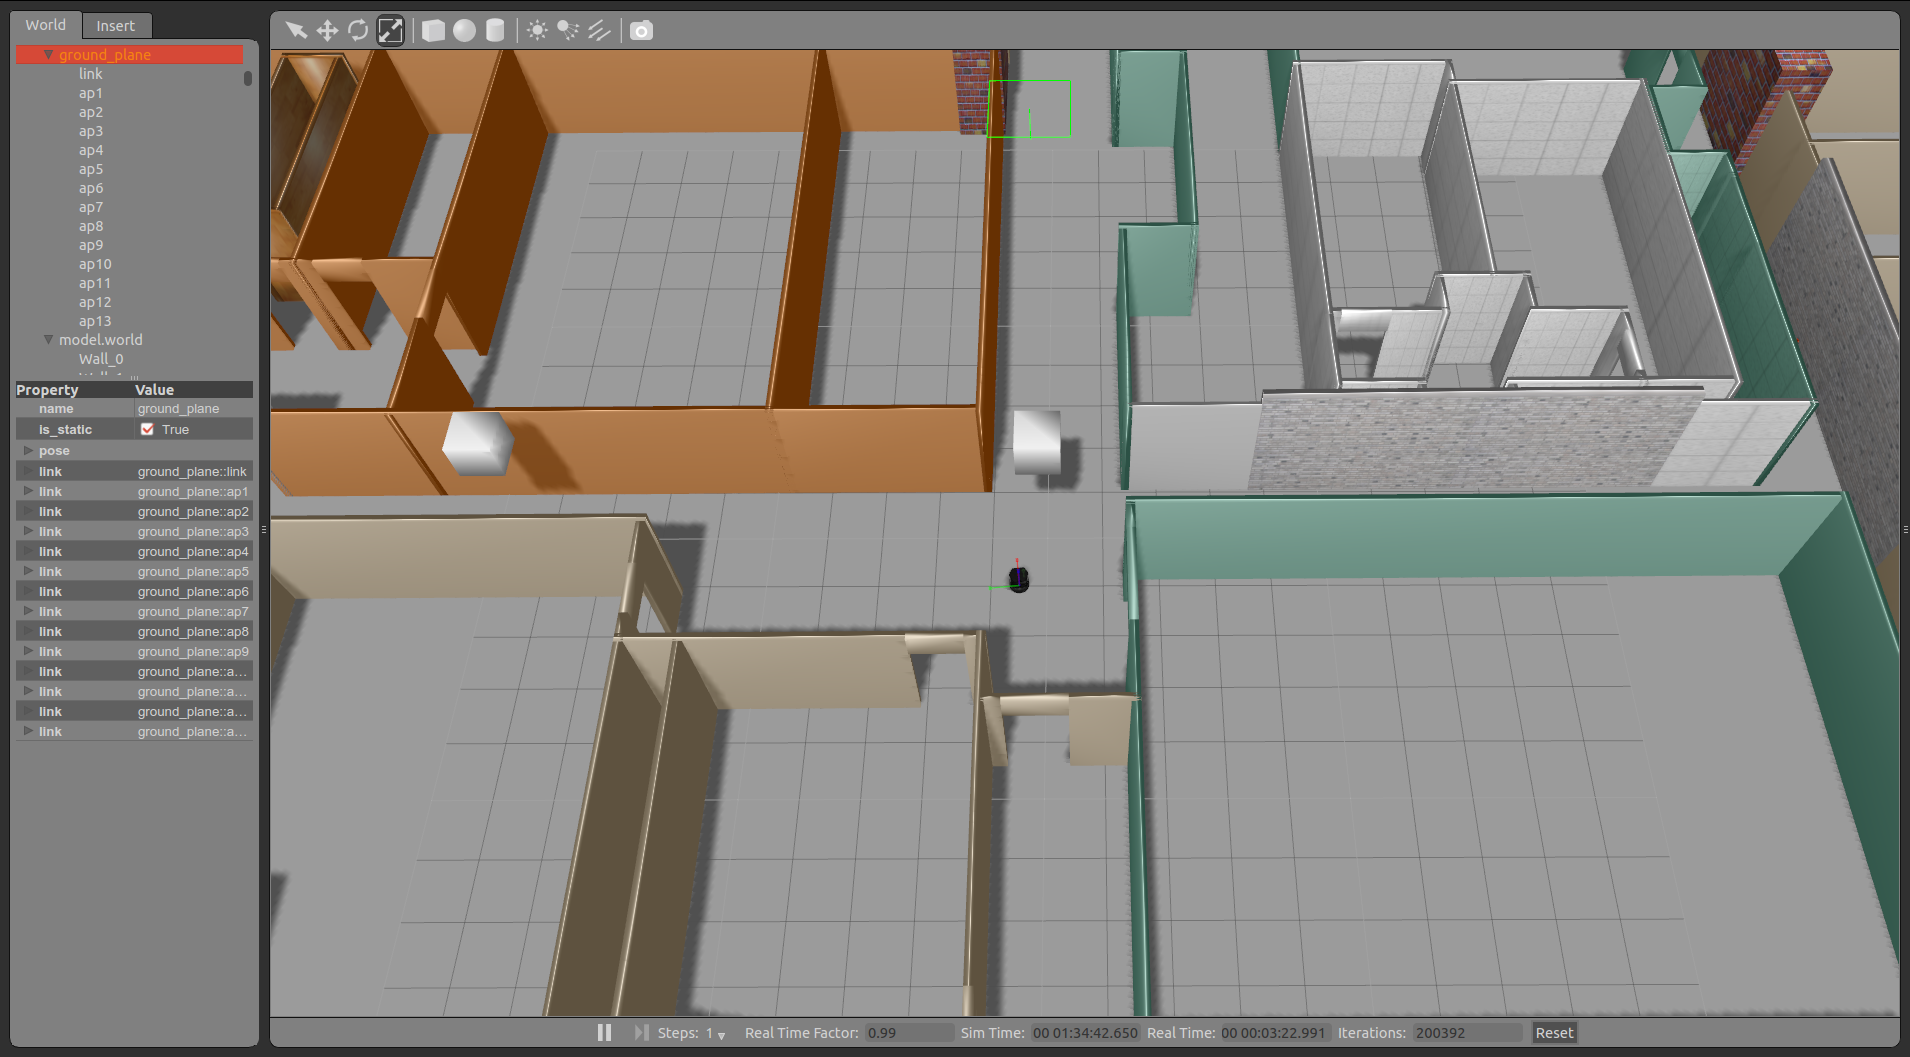
\includegraphics[width=\textwidth]{images/gazebo.png}
		\label{subfig:a}
		\caption{}
		\vspace{2em}
	\end{subfigure}
	\begin{subfigure}[b]{\textwidth}
	    \centering
		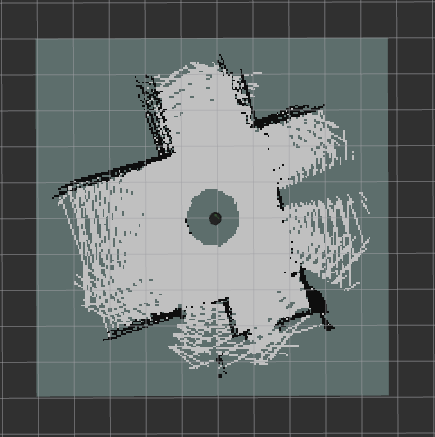
\includegraphics[width=0.75\textwidth]{images/gazebo1.png}
		\label{subfig:b}
		\caption{}
	\end{subfigure}
\caption{(A) Shows a simulation environment of Davis Hall, UB, created using Gazebo simulator for this work. (B) Shows the occupancy grid obtained from the vision sensor using RTAB-Map through topic /map\_explore.}
\end{figure*}

\par The consequent challenge is to identify the frontiers in the occupancy grid. As a part of solving an engineering issue discussed at the end of this chapter, we create a low resolution occupancy grid from the actual one every time it updates and frontiers are identified using the custom occupancy grid. Frontier is the boundary between explored i.e the grey cells and unexplored i.e the light blue cells. Each empty cell $v(m_i)=0$, is searched for at least one unknown cell $v(m_i)=-1$ adjacent to it and if found the cell is marked as a frontier cell given by,
\begin{equation}
    F = \{c^{[xy]} | c^{[xy]} \in O, \exists c^{[(x+m)(y+n)]} : p(c^{[(x+m)(y+n)]})=0.5, m\in[-1,1], n\in[-1,1]\}
\end{equation}
% The following the pseudo code to identify the grid cells which form the boundary separating the unknown from the free/empty space. 
The compute\_frontiers method in the controller.py node subscribes to the /map\_explore topic published by mapping.launch of RTAB-Map and detects the frontier cells.

\section{Information gain}
Entropy is the measure of uncertainty or randomness. Conditional entropy is defined as the entropy of a conditional distribution\cite{15}. The motto of exploration is to minimize the expected entropy of the belief as quickly as possible. As discussed in chapter 2, the following computes the expected entropy at a grid cell. 

\begin{equation}
    H = -\sum_{c^{[xy]}}[p(c^{[xy]})log_p(c^{[xy]}) + (1-p(c^{[xy]}))log(1-p(c^{[xy]}))], where~c^{[xy]} \in F
\end{equation}

We now calculate the cost for visiting each frontier cell. The cost in our case is simply the euclidean distance between robots position r and the target cell and is given by,

\begin{equation}
    \|C\|_{[xy]} = d(c^{[xy]},r^{[xy]}), where~c^{[xy]} \in F
\end{equation}
The optimal information gain associated with each frontier cell is defined as the difference between the expected entropy at it and the cost to visit it and is given by

\begin{equation}
    G_{[xy]} = H_{[xy]} - C_{[xy]} 
\end{equation}

\section{Frontier Allocation}
This work presents a new frontier allocation strategy which uses signal strengths from Wi-Fi routers. The proposed strategy is compared with another benchmark frontier allocation like optimal gain which are discussed in chapter 2. Wi-Coverage based frontier allocation provides a systematic coverage compared to the other approach.

\par To describe Wi-Coverage algorithm we consider two APs with access point IDs AP1 and AP2. We assume these APs are placed in an empty, obstacle free space as shown below in Fig 3.2. The rectangle with solid outline is the test environment and small green cubes represent the APs. Blue dotted circular outlines represent the reach of each APs and the dotted line between them divides the regions of AP dominance assuming such signal strength model. In other words, if the robot sensing Wi-Fi is in the region right to the line, it senses a stronger signal from AP1 than AP2. Similarly if it moves over the line towards AP2, it understands that the current region is dominated by AP2 than other APs which is only AP1 in this case. It is this ability to sense the dominance of APs in every region of the environment which forms the basis of Wi-Coverage of clustering the space online i.e. without any prior availability of clustered regions. The dividing line shown is only for illustration purposes and no such information about APs or the environment is required for Wi-Coverage. 

\begin{figure*}
    \begin{subfigure}[b]{0.495\textwidth}
		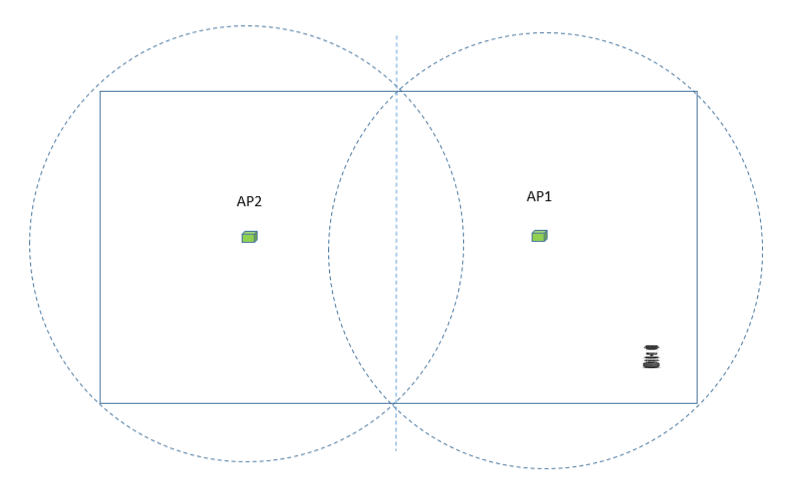
\includegraphics[width=\textwidth, height=0.6\textwidth]{images/w1.png}
		\label{subfig:a} 
		\caption{}
	\end{subfigure}
	\begin{subfigure}[b]{0.495\textwidth}
		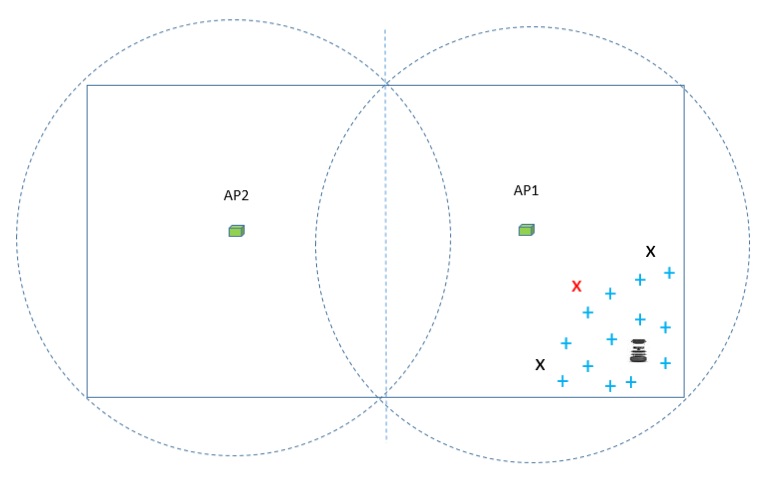
\includegraphics[width=\textwidth, height=0.6\textwidth]{images/w2.png}
		\label{subfig:b}
		\caption{}
	\end{subfigure}
	\begin{subfigure}[b]{0.495\textwidth}
		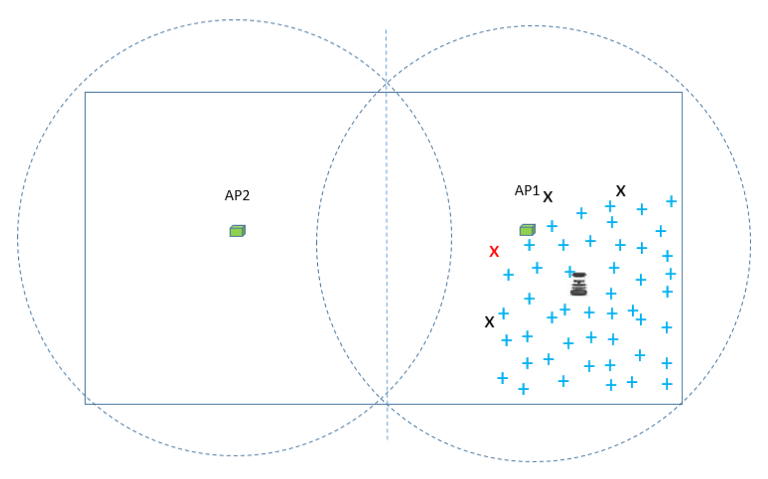
\includegraphics[width=\textwidth, height=0.6\textwidth]{images/w3.png}
		\label{subfig:c} 
		\caption{}
	\end{subfigure}
	\begin{subfigure}[b]{0.495\textwidth}
		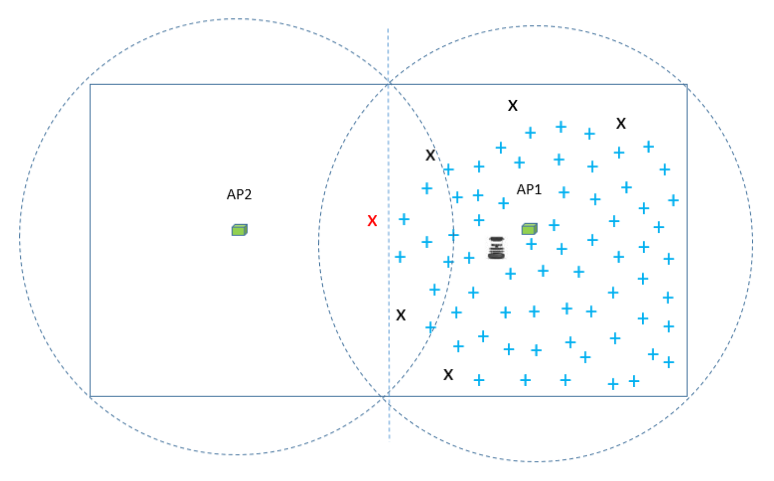
\includegraphics[width=\textwidth, height=0.6\textwidth]{images/w4.png}
		\label{subfig:d}
		\caption{}
	\end{subfigure}
    \begin{subfigure}[b]{0.495\textwidth}
		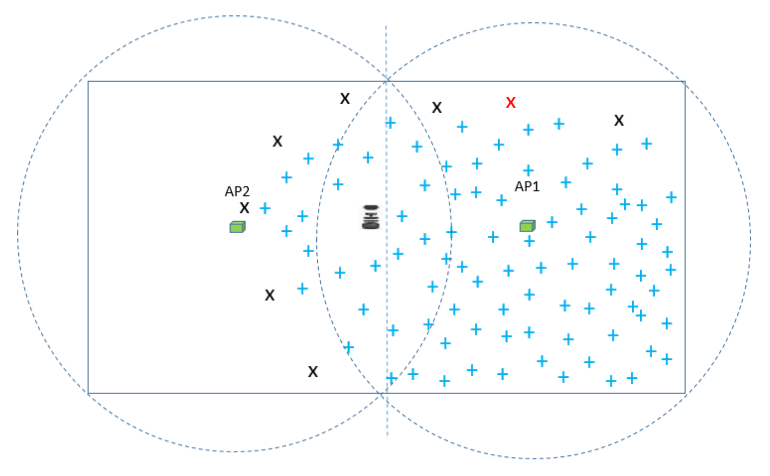
\includegraphics[width=\textwidth, height=0.6\textwidth]{images/w5.png}
		\label{subfig:e} 
		\caption{}
	\end{subfigure}
	\begin{subfigure}[b]{0.495\textwidth}
		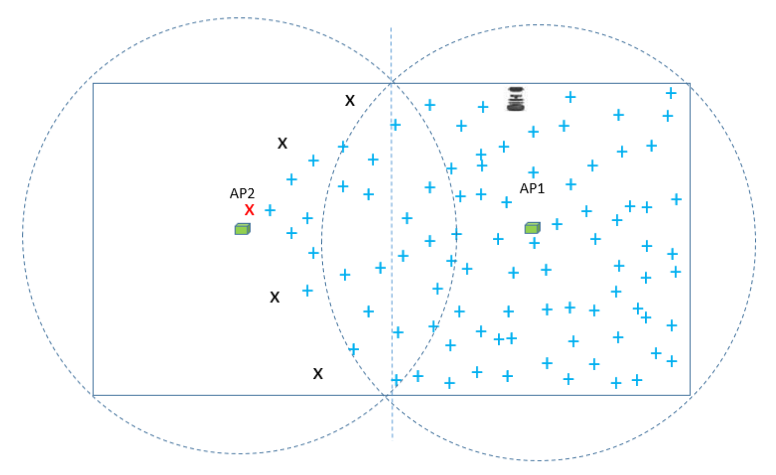
\includegraphics[width=\textwidth, height=0.6\textwidth]{images/w6.png}
		\label{subfig:f}
		\caption{}
	\end{subfigure}
    \begin{subfigure}[b]{0.495\textwidth}
		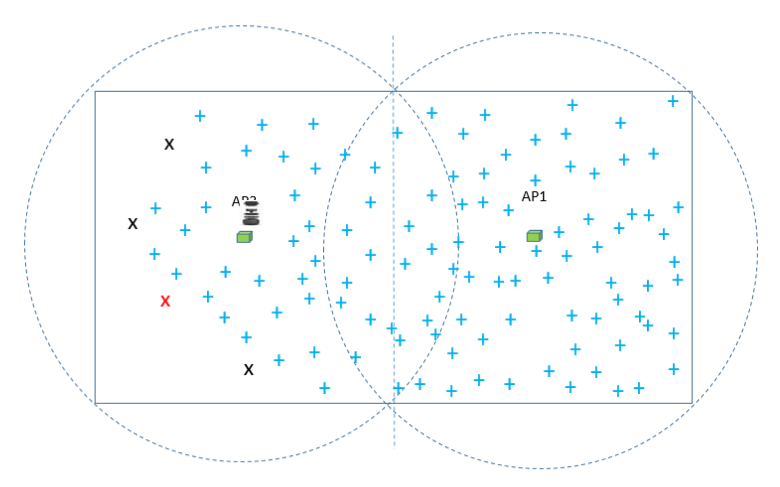
\includegraphics[width=\textwidth, height=0.6\textwidth]{images/w7.png}
		\label{subfig:g} 
		\caption{}
	\end{subfigure}
	\begin{subfigure}[b]{0.495\textwidth}
		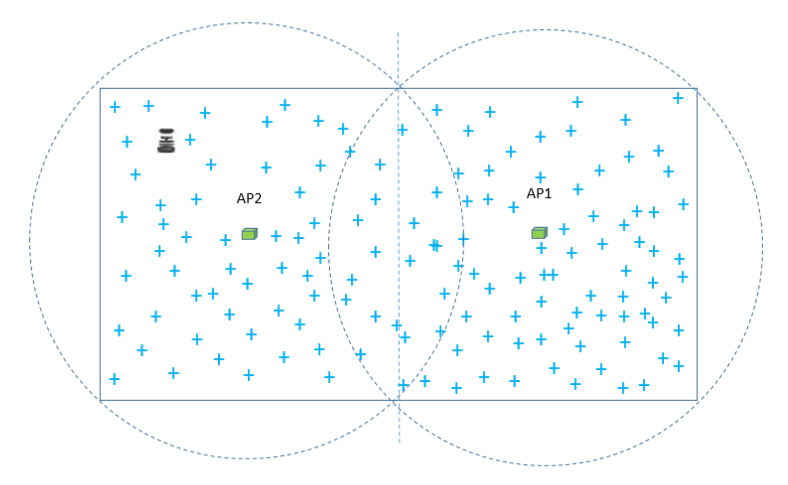
\includegraphics[width=\textwidth, height=0.6\textwidth]{images/w8.png}
		\label{subfig:h}
		\caption{}
	\end{subfigure}
\caption{Illustration of Wi-Coverage in a rectangular space with two access points. + - explored area, x(black) - frontiers identified, x(red) - frontier picked, AP1 and AP2 are access points}
\end{figure*}

\par The robot does an initial Wi-Fi scan and initializes expoAP, which holds the cluster ID(AP ID itself) being explored,to the strongest AP ID which we call the dominant AP. A $360^o$ sensor sweep is performed by the robot and frontiers are obtained using the above explained method exploring partially the environment as shown in Fig 3.2 (A). The explored space is represented in '+' and the white space in the environment represents the area to be explored. The frontier poses are then processed through a Priority Queue which heaps them based on their respective information gain and are associated to currdomAP, the current dominant AP. The Queuer then pops the best frontier associated with expoAP shown in red 'x' and the robot plans its path and moves to it. The robot performs a Wi-Fi scan along with the sensor sweep. If the current dominant AP is same as expoAP, new frontiers are queued and associated with the same AP repeating the above process as illustrated in Fig 3.2 (C) and (D). The robots continues to explore the same fashion until it finds itself sensing better of another AP apart from expoAP as shown in Fig 3.2 (E). Here the Turtlebot crosses the imaginary line of dominance and experiences a stronger signal strength from AP2 and hence the current dominant AP is changed to AP2 ID while expoAP remains unchanged. At this juncture, all new frontiers detected after the sensor sweep are queued in to the Priority Queue and are associated to the currdomAP which is this time, AP2. The frontier popped by the queuer is associated with expoAP i.e AP1 and has the highest of information gains compared to its members. Hence the robot instead of visiting a frontier else where, it visits the frontiers remaining in the partially explored cluster as shown in the Fig 3.2 (F). This continues until all the frontiers associated with expoAP are visited thereby completely exploring the cluster. It is important to note that all new frontiers identified while exhausting the current cluster are associated with their respective cluster numbers along with their information gains. Also the cost to visit the frontiers which are already queued are always updated at each sensor sweep. Once all frontiers corresponding to expoAP are exhausted, it is updated to another cluster ID whose sum of expected gains of all its  frontiers are the maximum. In this case its updated to AP2 ID which is the only remaining cluster. The frontier popped is visited as shown in Fig 3.2 (G) and all new frontiers identified are associated with expoAP, which is now AP2. The process is repeated until all frontiers are visited thereby exploring the entire environment as shown in Fig 3.2 (H). The following is the pseudo-code of Wi-Coverage implementation for a single robot.\\
\vspace{1mm}\\

\noindent\textbf{Algorithm 1: Wi-Coverage using single robot}\\

\begin{algorithm}[H]
% \caption{Wi-Coverage}
\KwData{\\
WiFiC() : get list of AP ids with SS from reachable APs\\
Q() : pushes, pops and heaps}
\textbf{initialize} expoAP \gets $AP\_id\_with\_max\_RSS$\\
\While{no frontiers found}{
\While{!Q(expoAP) is empty}{
O \gets getOccupancyGrid()\;\\
F \gets getFrontiers(G)\;\\
E \gets computeEntropy(F)\;\\
C \gets computeCost(F)\;\\
G \gets computeInfoGain(F)\;\\
Z \gets WiFiC()\;\\
currdomAP \gets getdominantAP(Z)\; \\
Update\_Queue : Q(currdomAP).heap(G, F) \\
nextpose \gets Q.pop(Q(expoAP))\\
}
expoAP \gets $AP\_id\_with\_max(sum(G))$\;\\
}
\end{algorithm}

\vspace{4mm}
\section{Multi-Robot Scenario}
In addition to coverage problem, another reason for the extensive research in autonomous exploration is the benefit that tasks yield when scaling up the number of robots. In many cases multiple robots prove efficient in exploration since huge amounts of time can be saved especially in sizable environments. In case of multiple robots to perform the above discussed frontier exploration, the following should be accomplished for unknown environments.
\begin{itemize}
    \item \textbf{SLAM modules} : Each robot should have its own SLAM module. In other words, they should individually map and localize in their respective local maps.
    \item \textbf{Frontier Detection} : All robots perform frontier exploration for which the frontiers are identified using the above discussed methods. This module is integrated into each robot's controller independently. 
    \item \textbf{Map merging} : As each robot gains information about the environment around itself resulting in a local map, all maps are merged using algorithms such as Graph SLAM\cite{25}.
    \item \textbf{Cluster allocation}: Wi-Coverage works independently on each robot in case of allocating frontiers such that the robot covers the environment cluster by cluster. But in multi robot case, a centralized control is necessary to assign clusters to the robots. This control also checks the number of robots being deployed on the field, especially when the number of robots available are greater than the clusters to be explored.
\end{itemize}

\par When multiple robots are available, clustering the environment online becomes an ultimate advantage. Traditional methods such as cellular decomposition approaches cluster the environment but require complex computations to be performed. Some also expect the robot to remember the visited  spaces which needs storage and solving of necessary edge cases. Wi-Coverage is free from such limitations and prerequisites.      
It can be observed that in case of random frontier allocation, the efficiency of exploration is poor and robots trajectory is completely unpredictive. In a multi robot scenario, though robot coordination becomes easier since the basic criteria of "no two robots get the same frontier" is only to be followed, this strategy still performs poor since robots generally end up with longer trails. Also the number of robots effect the exploration time and computation cost.

\begin{figure*}
    \begin{subfigure}[b]{0.495\textwidth}
		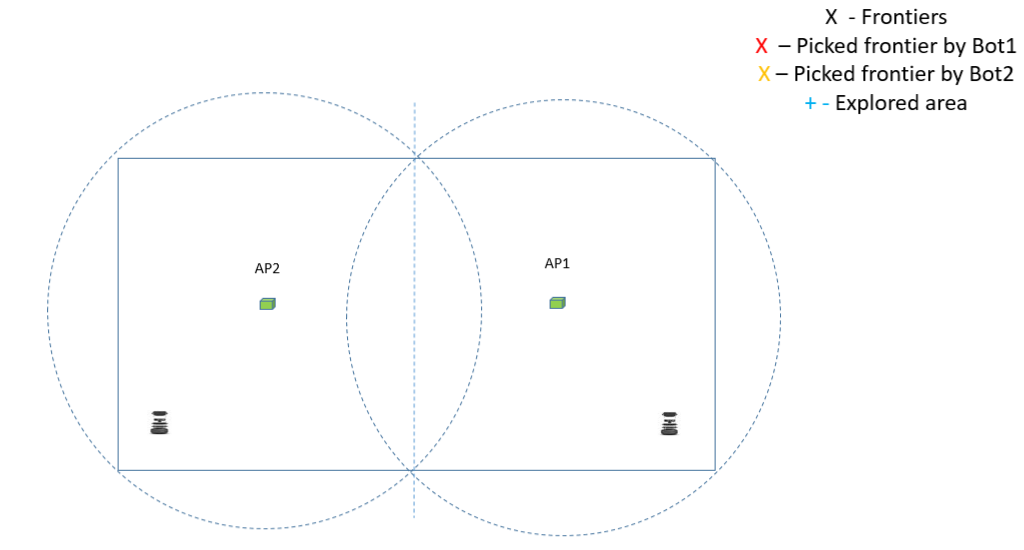
\includegraphics[width=\textwidth, height=0.6\textwidth]{images/wm1.png}
		\label{subfig:a} 
		\caption{}
	\end{subfigure}
	\begin{subfigure}[b]{0.495\textwidth}
		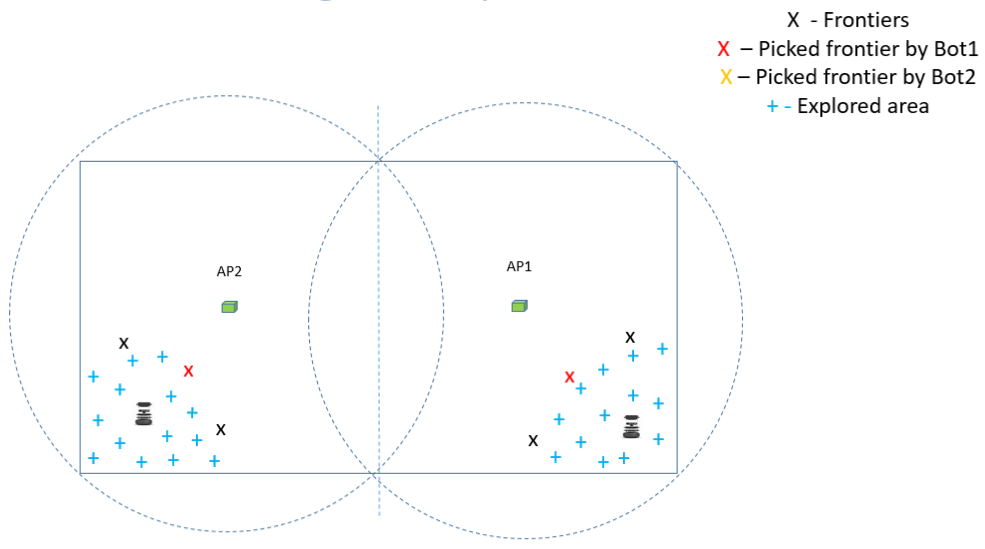
\includegraphics[width=\textwidth, height=0.6\textwidth]{images/wm2.png}
		\label{subfig:b}
		\caption{}
	\end{subfigure}
	\begin{subfigure}[b]{0.495\textwidth}
		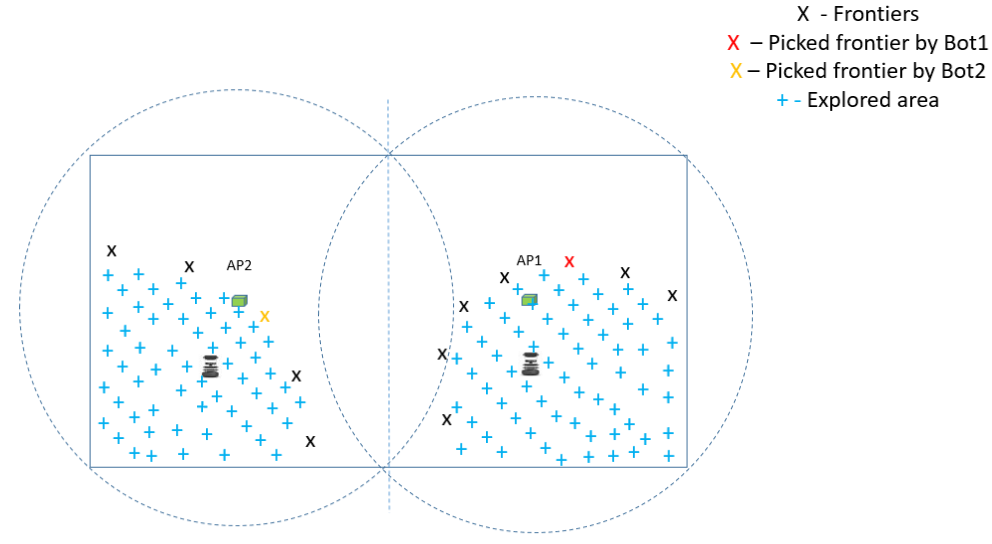
\includegraphics[width=\textwidth, height=0.6\textwidth]{images/wm3.png}
		\label{subfig:c} 
		\caption{}
	\end{subfigure}
	\begin{subfigure}[b]{0.495\textwidth}
		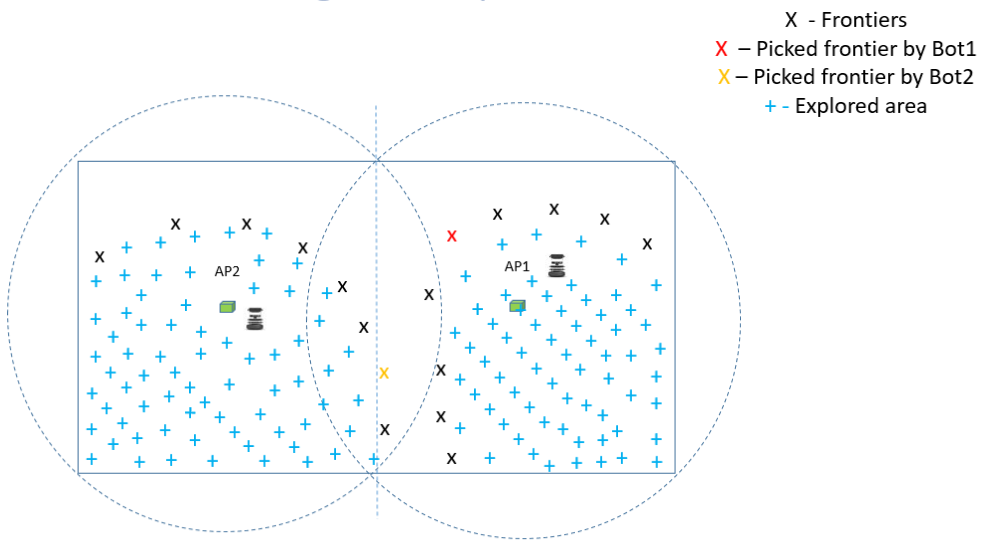
\includegraphics[width=\textwidth, height=0.6\textwidth]{images/wm4.png}
		\label{subfig:d}
		\caption{}
	\end{subfigure}
    \begin{subfigure}[b]{0.495\textwidth}
		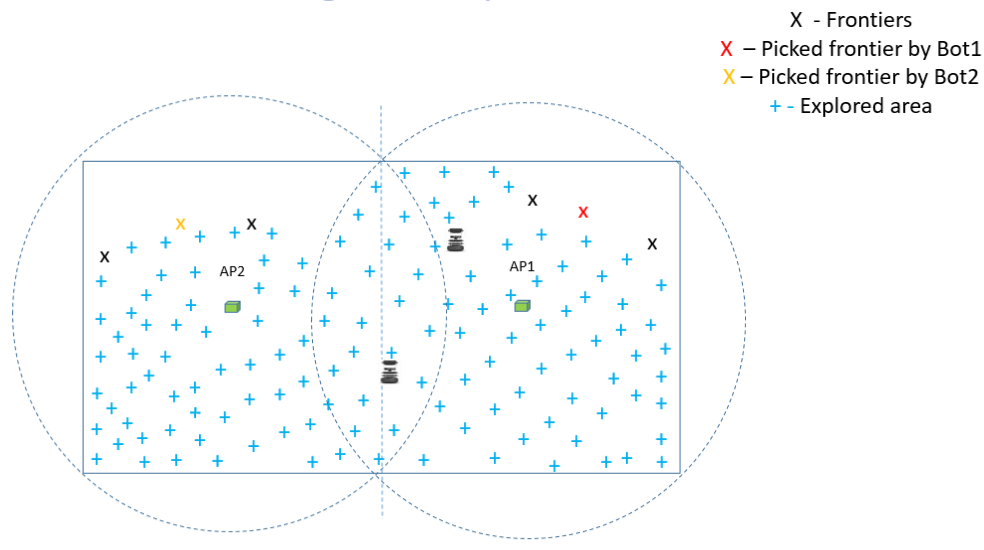
\includegraphics[width=\textwidth, height=0.6\textwidth]{images/wm5.png}
		\label{subfig:e} 
		\caption{}
	\end{subfigure}
	\begin{subfigure}[b]{0.495\textwidth}
		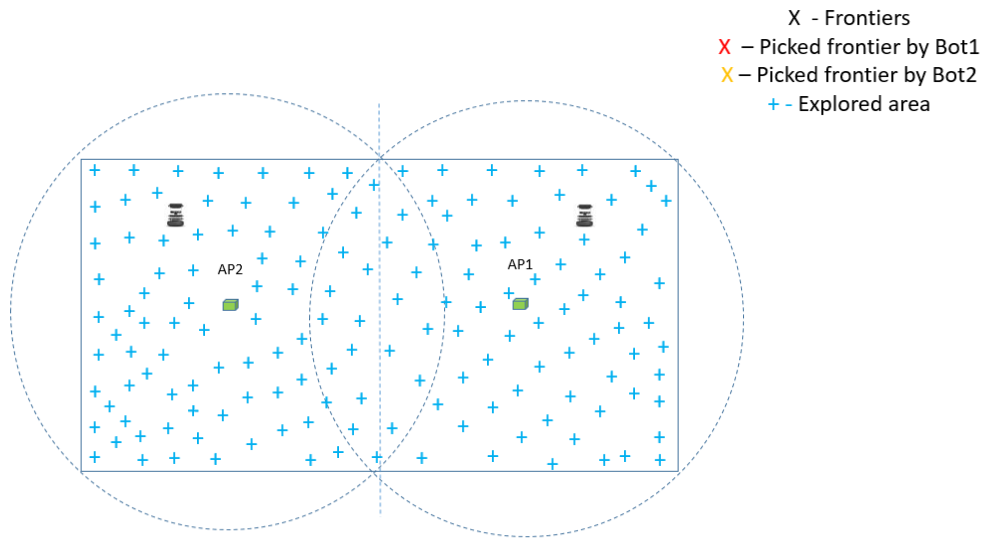
\includegraphics[width=\textwidth, height=0.6\textwidth]{images/wm6.png}
		\label{subfig:f}
		\caption{}
	\end{subfigure}
%     \begin{subfigure}[b]{0.495\textwidth}
% 		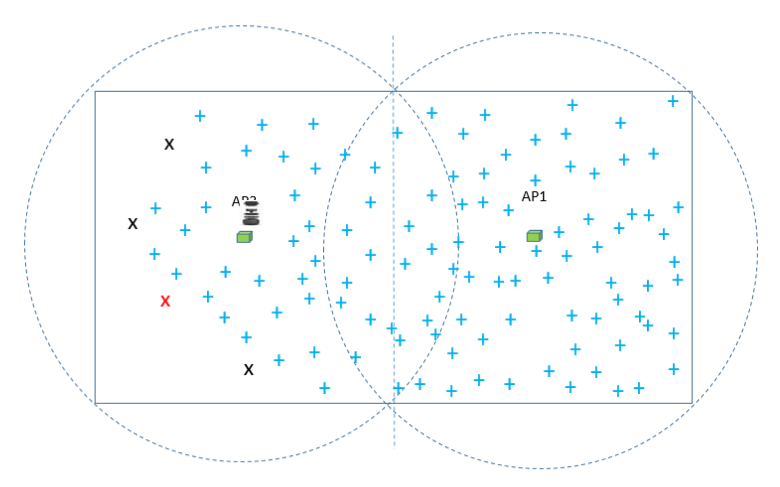
\includegraphics[width=\textwidth, height=0.6\textwidth]{images/w7.png}
% 		\label{subfig:g} 
% 		\caption{}
% 	\end{subfigure}
% 	\begin{subfigure}[b]{0.495\textwidth}
% 		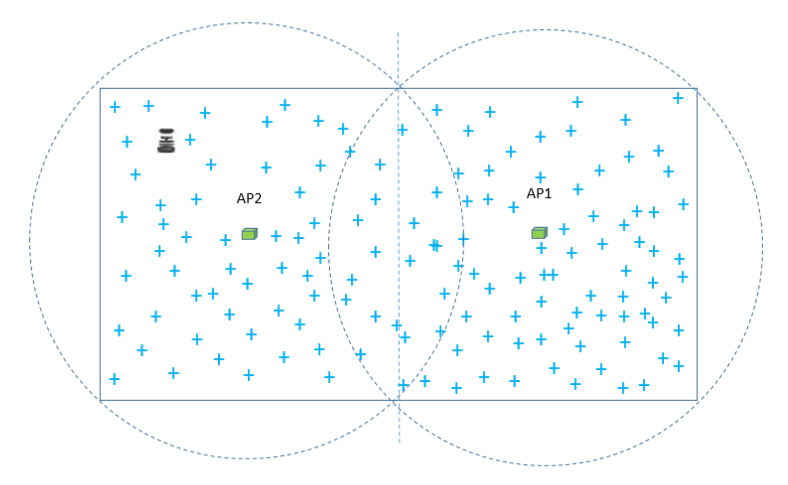
\includegraphics[width=\textwidth, height=0.6\textwidth]{images/w8.png}
% 		\label{subfig:h}
% 		\caption{}
% 	\end{subfigure}
\caption{Illustration of Wi-Coverage with multiple robots in a rectangular space with two access points.}
\end{figure*}

In case of multi-robots, Wi-Coverage has various advantages over other traditional methods.
\begin{itemize}
    \item \textbf{Coordination strategy}: In traditional coverage strategies, the robots need to communicate their poses and the local maps they have explored which can be represented by various metrics(see Chapter 2). In general, these maps, especially the point clouds are data rich and transferring such data takes a toll on the network. Though converting them to relatively simpler structures like graphs or Voronoi diagrams would help reduce the traffic in the network, additional nodes are required to process them continuously. Also as the environment grows larger, the transfers become costly.
    
    \item \textbf{Resource management}: Most coverage methods have a generic strategy which uses all the available robots to explore the environment. Using such methods in scenarios where resources are abundant than required, needs special actions of not exploiting them. Wi-Coverage takes into consideration such requirements by allowing only sufficient work force rather than deploying all the available robots on the field. 
\end{itemize}

To describe Wi-Coverage in a multi-robot scenario, consider the previous environment shown in Fig 3.2(A) but with two robots placed in the environment as shown in Fig 3.3(A). Each robot is equipped with the same sensors, a controller and a motion planner. A master robot allocates clusters to all the robots in the environment. It also decides whether a robot is to be deployed for exploration on the field. Once a robot is allocated a cluster, it explores the environment using Wi-Coverage described in Algorithm 1. 
\par After an initial scan for Wi-Fi APs, the master robot which we call the Allocator gets updated of the total number of APs listened to. It then assigns a cluster to each robot based on its dominant AP. In our example, Robot 1 to the right is assigned cluster AP1 and Robot 2 is assigned cluster AP2 since they are the corresponding dominant APs they listen to. The Allocator maintains a record of the allocated clusters and unallocated clusters in the environment. The robots then perform exploration using Wi-Coverage in their respective clusters as shown in the Fig 3.3 (C),(D) and (E). Once the clusters are explored, the Allocator is updated by sending a feedback message from each robot. If any unexplored cluster is available, the Allocator assigns the cluster to the robot which listens to the corresponding AP, the strongest. Algorithm 2 below shows a pseudo-code for Wi-Coverage using multiple robots.
% \clearpage
\vspace{1.5em}

\noindent\textbf{Algorithm 2: Wi-Coverage using multiple robots}

\begin{algorithm}[H]
% \caption{Wi-Coverage}
\KwData{\\
WiFiC() : gets AP ids with SS of reachable APs\\
Q() : pushes, pops and heaps\\
Allocator() : Assigns clusters}
\textbf{initialize};
clusterlist \gets UnionOfAPidsSensed\\
\While{!clusterlist is empty}{
\For{each bot}{
    bot(expoAP) \gets Allocator() assigns cluster_i\\
    \While{$!cluster_i$ is explored}{
        do \textbf{Algorithm 1}\\
    }
    clusterlist \gets delete $cluster_i$\\
    \If {new AP detected}{
    clusterlist \gets $new\_cluster$\\
    }
}
}
\end{algorithm}

\vspace{1.5em}

\par The Allocator also considers situations when more than one robot gets the same cluster to be explored. This happens when robots share the same dominant AP, i.e when they start from the same cluster. In such case, the robot which listens stronger to the AP gets the current cluster and the other bot(s) get(s) the cluster(s) to which it(they) listen the best apart from the current AP as shown in Algorithm 3 below.

\vspace{1.5em}

\noindent\textbf{Algorithm 3: Cluster allocation}

\begin{algorithm}[H]
% \caption{Wi-Coverage}
% \KwData{\\
% % Allocator() : tracks cluster allocation
% N : Number of robots}
\While{no frontiers found}{
\For{each update}{
    % \For{i=1\,1$<$N-1}
    \If{bot_i(expoAP)~ $==$~ bot_{j}(expoAP)}{
        min(SS_i,SS_{j}) \gets $corresponding\_next\_best\_domAP$\;\\
    }
}
}
\end{algorithm}

Algorithm 4 shows a psuedo-code describing the frontier selection of a robot in seek of the cluster assigned. In the above scenario where robots start from same dominant AP region, the robot which is assigned another cluster selects frontiers such that it moves towards by tracking the signal strength.\\

\noindent\textbf{Algorithm 4: Cluster search when bots start from same location}

\begin{algorithm}[H]
% \caption{Wi-Coverage}
\KwData{\\
\%SS(): gets percentage signal strength}
\While{!\%SS(expoAP) $>$ 0}{
nextpose \gets maximize(SS(Q.pop(Q(domAP))))\;\\
}
\end{algorithm}

If no unexplored clusters are available and all which were assigned are explored, the exploration is said to be complete as shown in Fig 3.3(F). The maps from each robot are then merged using Graph SLAM.
To summarize, the robots perform exploration using Wi-Coverage individually in clusters assigned by the Allocator. Since the robots need not know each others positions, the only information transferred between the robots is merely a cluster id while allocating clusters. This is far less complicated and less communication intensive than other available methods for multi-robot exploration.

% \clearpage

\section{Systems}
This section is about the software and hardware systems used in this work. Hardware design, communication protocols, middleware design and structure and about simulation software, Gazebo are discussed.  

\lhead{\emph{Systems}}
\subsection{Hardware and low-level drivers}
The lowest layer of system abstraction is the hardware. The motorized wheel, all hard connections which carry power and data in and around the robot, the sensor payloads and the batteries come under this.
Sensors communicate using various protocols and over different hardware interfaces. The interface between low-level drivers and the middleware translates the raw data from the sensors into a common format which is used by other consequent processes.

\begin{figure}[!b]
    \centering
    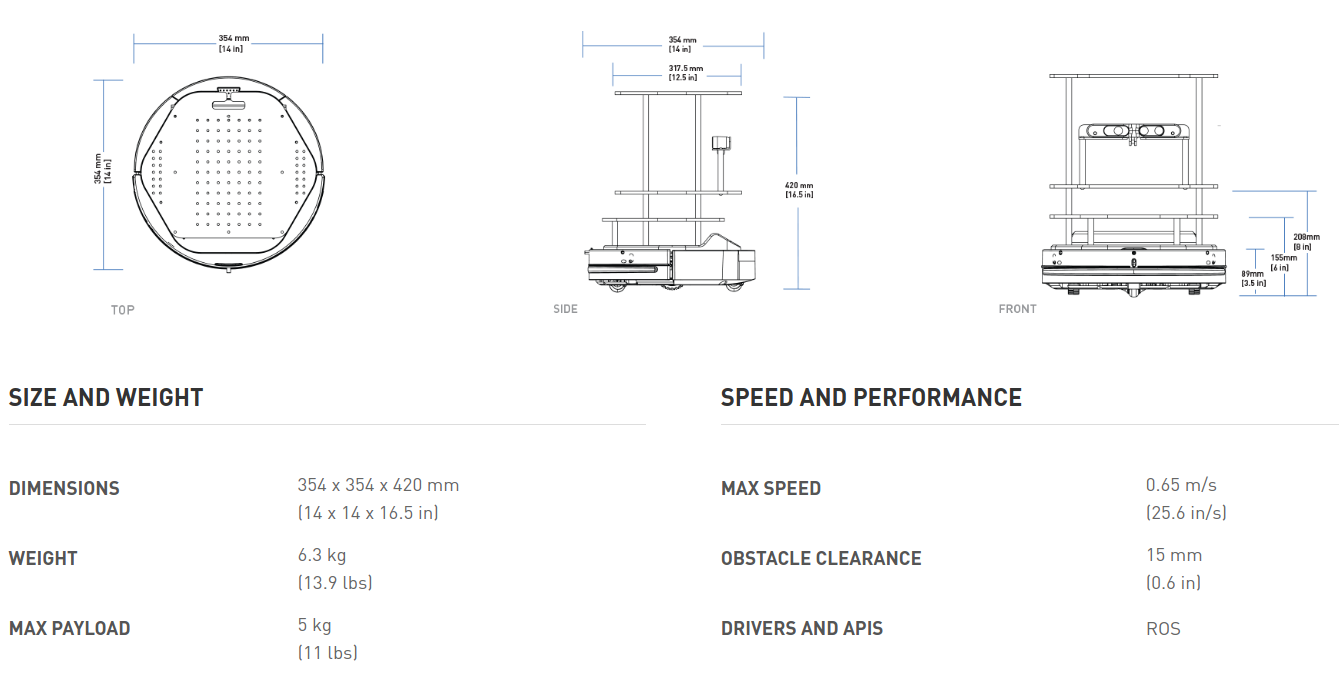
\includegraphics[width=\textwidth]{images/botspecs.png}
    \caption{Turtlebot 2 technical specifications. Image courtesy \cite{41}}
    \label{fig:tb}
\end{figure}

\subsubsection{Darwin}
Our robot, Darwin, which we choose to make it into an autonomous explorer is a Turtlebot 2. Turtlebots are low-cost, personal robot kits with open-source software created by Willow Garage by Melonee Wise and Tully Foote\cite{32}. Darwin is the next and improved version of the first generation Turtlebot developed by Clearpath Robotics. A Turtlebot has been built for ROS and supports all major packages out of the box. As with many other ROS platforms, one of the biggest strengths of the Turtlebot is the support community. Fig 3.4 below lists the specifications of the robot. Darwin is equipped with an Yujin Kobuki mobile base, a Kinect Xbox 360 sensor, an Nvidia TK1 CPU which contains our code base, fast charger and a 2200mAh battery pack. It also comes with a fast charging dock that Turtlebot can autonomously dock with. All low level drivers that handle wheel motors, encoders and other communication protocols are built-in.

\section{Middleware and High-level applications}
The low-level hardware such as motors or cameras and high-level applications such as motion planning or object recognition are integrated by a middleware. It is a software layer facilitating communication between them which is required for modularising components in a robot system.   

\subsection{ROS: Robot Operating System}
Nowadays autonomous Robots are getting more and more complex, using various types of sensors and motors\cite{20}. Therefore the demand for a framework that integrates the sensors and all the hardware components of the robot with an operating system is quite high. Another need for the community is code re-usability. ROS is an open source framework\cite{13} that aids in development of various robot applications. It serves as a platform which eliminates the work of building an application from scratch by providing various low level drivers and communication protocols. It makes a developer's work much easier and focused on the core application and saves considerable amount of time. Apart from offering quality applications as packages which are a run and play type, it hosts a great community which helps solve problems.
\par ROS is also popular as a meta-operating system that provides tools and libraries to help the users develop complex robotic applications. It supports parallel computing and distributed communication framework. The individual components in an application can interact using ROS without being constrained to run on a single computer. Although there are various robot frameworks such as Player, YARP, Orocos, CARMEN, Orca, MOOS, and Microsoft Robotics Studio available, ROS has gained attention due to its distributed nature, code re-usability and community support.

\subsection{ROS Levels}
ROS uses divide and conquer method while designing complex robot applications\cite{34}. Nodes are the fundamental components of ROS. These are individual executables which communicate with each other through messages using topics as shown in Fig 3.6. Though ROS is not a full fledged operating system, the primary idea behind this is to emulate such behavior while promoting code reuse and distributed networking. Nodes are contained in a package and packages with common goal are grouped as stacks such as navigation stack. Each package has a manifest(\textit{package.xml}) that describes its functionality and dependencies on other packages. Fig 3.5 represents the communication framework of ROS\cite{33}.
The following describe various levels and components in ROS framework.

\begin{figure}[!b]
    \centering
    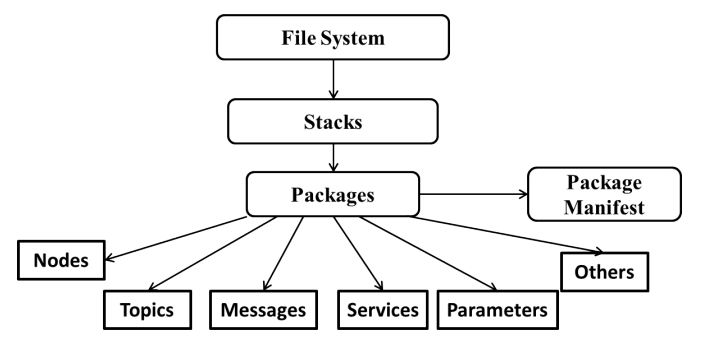
\includegraphics[width=\textwidth]{images/ros1.png}
    \caption{ROS as an ecosystem. Image from \cite{49}}
    \label{fig:r1}
\end{figure}

\begin{figure}[!b]
    \centering
    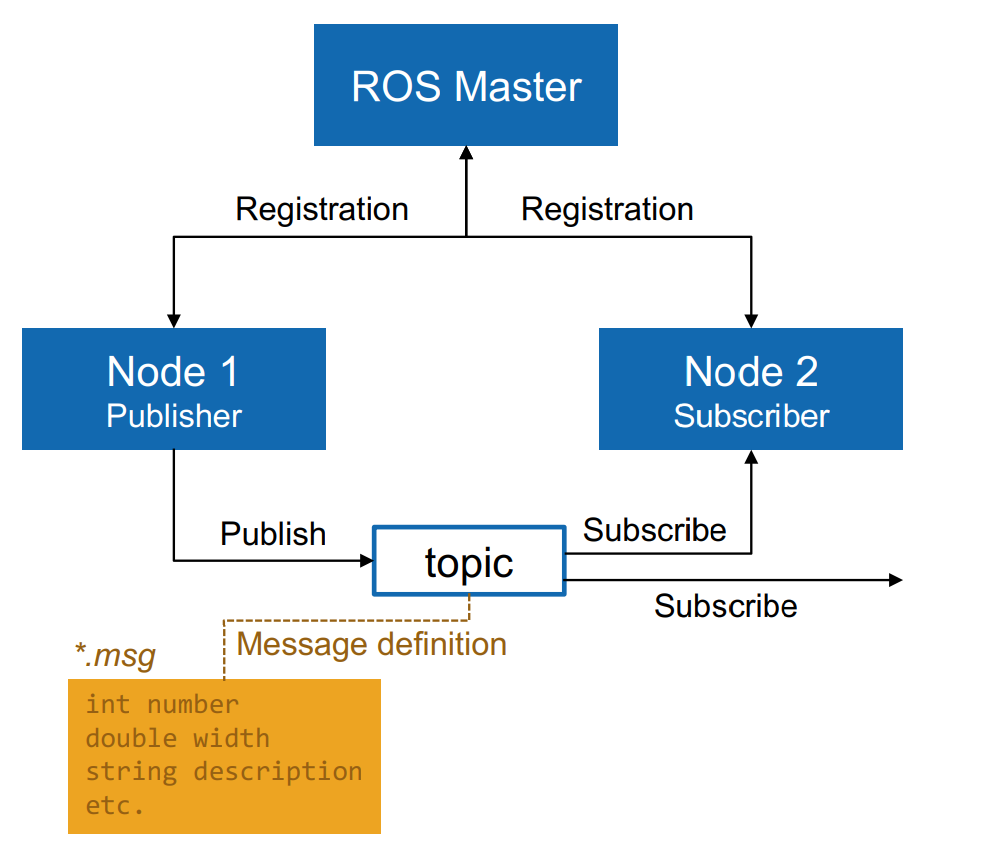
\includegraphics[width=0.75\textwidth]{images/ros2.png}
    \caption{Basic communication framework in ROS. Image from \cite{48}}
    \label{fig:r2}
\end{figure}

\subsubsection{File System Level}
\begin{itemize}
    \item Packages: These constitute the main unit for organizing software in ROS\cite{48}.
    \item Manifests: These provide metadata about a package, including its license information and dependencies, as well as language specific information such as compiler flags.
    \item Stacks: Collection of packages that provide aggregate functionality.
    \item Stack manifests: Similar to package manifests but provides data of the stack.
    \item Message: These are descriptions that define data structures for messages sent in ROS.\\ Example: \textit{my\_package/msg/MyMessageType.msg}.
    \item Service: These descriptions define the request and response data structures for services in ROS. This establishes a request and acknowledgement protocol between nodes to communicate efficiently. Example: \textit{my\_package/srv/MyMessageType.srv}.
\end{itemize}

\subsubsection{Computation Graph Level}
\begin{itemize}
    \item Nodes: Nodes are combined graphs which communicate via streaming topics, services and parameter server\cite{33}.
    \item ROS Master: This provides naming and registration services to the rest of the nodes in ROS system.
    \item Parameter Server: It is a shared, multi-variate dictionary that is accessible via network APIs. The parameter server is implemented using XMLRPC and runs inside of the ROS Master, which means that its API is accessible via normal AMLRPC libraries\cite{33}.
    \item Topics: These are named buses over which nodes exchange or share messages based on publish/subscribe policy.
    \item Bags: A format for saving and playing back ROS message data.
\end{itemize}

\subsection{Gazebo: Simulator}
Robot simulation is an essential tool in every roboticist's toolbox. A well-designed simulator makes it possible to rapidly test algorithms, design robots, perform regression testing, and train AI system using realistic scenarios. Gazebo\cite{18} is a 3D dynamic simulator with the ability to accurately and efficiently simulate populations of robots in complex indoor and outdoor environments. While similar to game engines, Gazebo offers physics simulation at a much higher degree of fidelity, a suite of sensors, and interfaces for both users and programs. The key features of Gazebo include\cite{18} multiple physics engines, a rich library of robot models and environments, a wide variety of sensors and convenient programmatic and graphical interfaces. Fig 3.5 above shows the building editor of Gazebo which just requires a blueprint of the environment to be created. Fig 3.8 shows the environment designed using the building editor. A blue print of the building was used and all measurements are to scale. Different colors are given to walls for better visual distinction. 

\begin{figure}
    \centering
    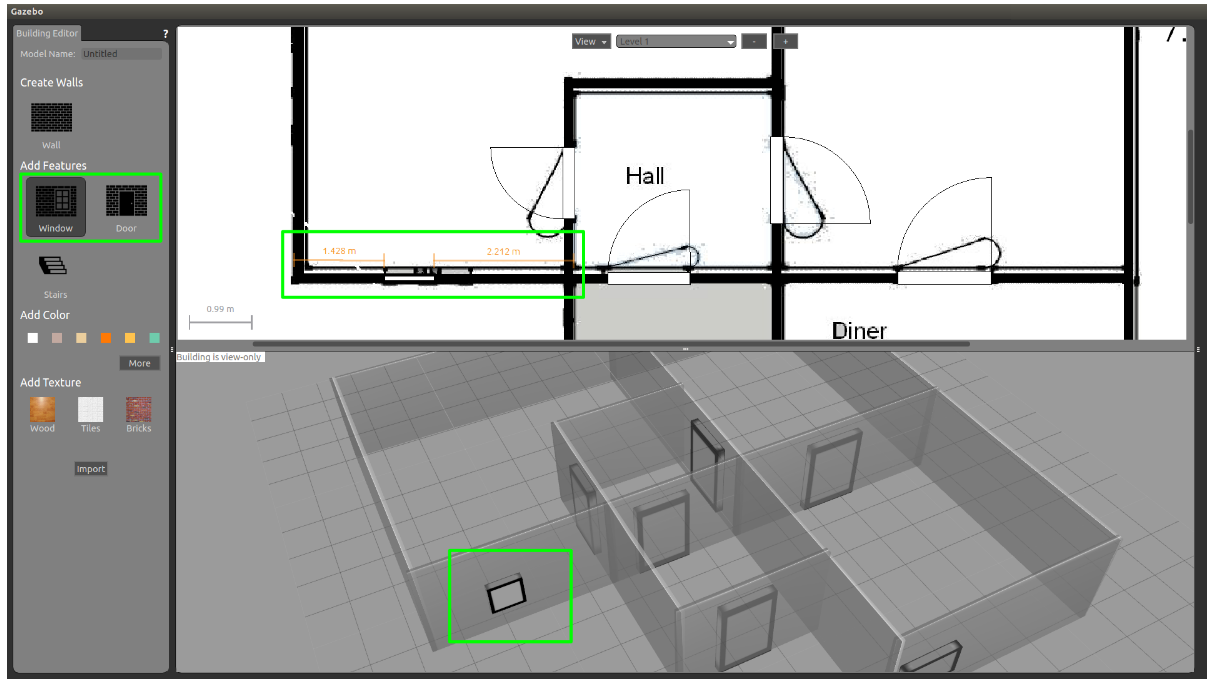
\includegraphics[width=\textwidth]{images/gazebo2.png}
    \caption{A snapshot of Gazebo simulator GUI. The interface shows the building editor where the top section is the blueprint and below is the environment being built using it.}
    \label{fig:gazebo}
\end{figure}

\begin{figure*}[!h]
    \begin{subfigure}[b]{\textwidth}
		\centering
		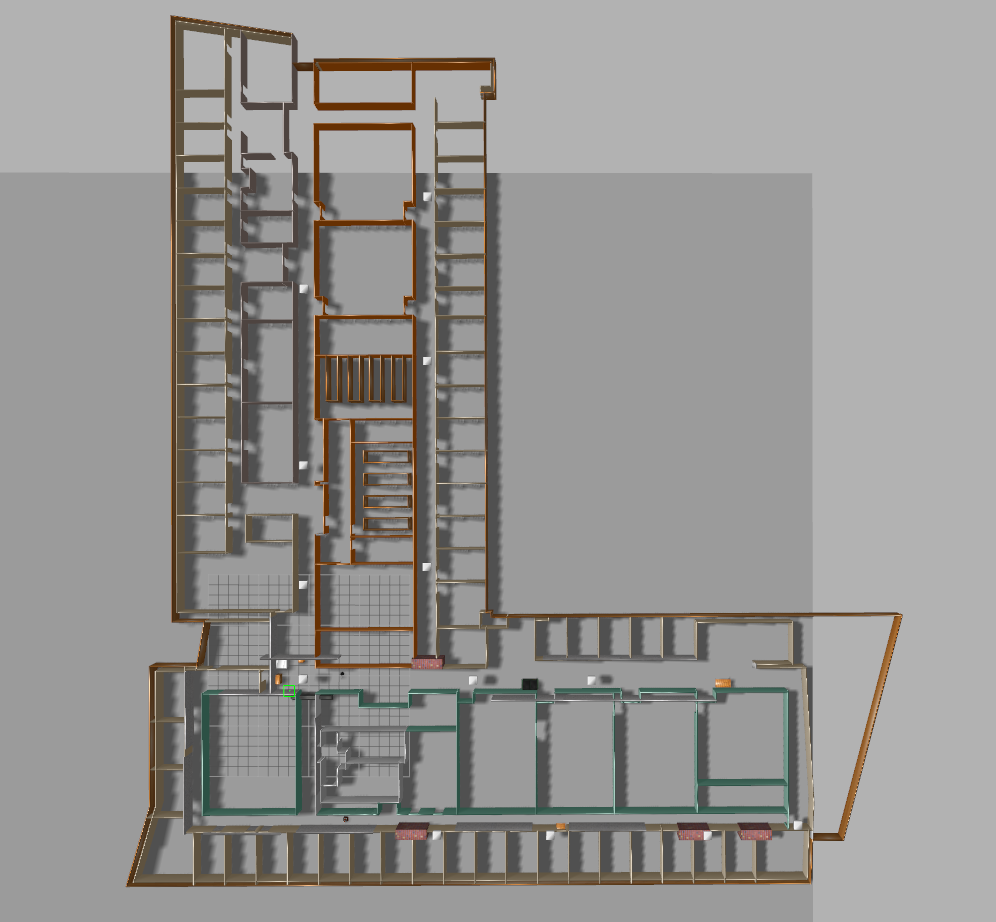
\includegraphics[width=0.49\textwidth]{images/davis3g1.png}
		\label{subfig:a}
		\caption{}
		\vspace{2em}
	\end{subfigure}
	\begin{subfigure}[b]{\textwidth}
	    \centering
		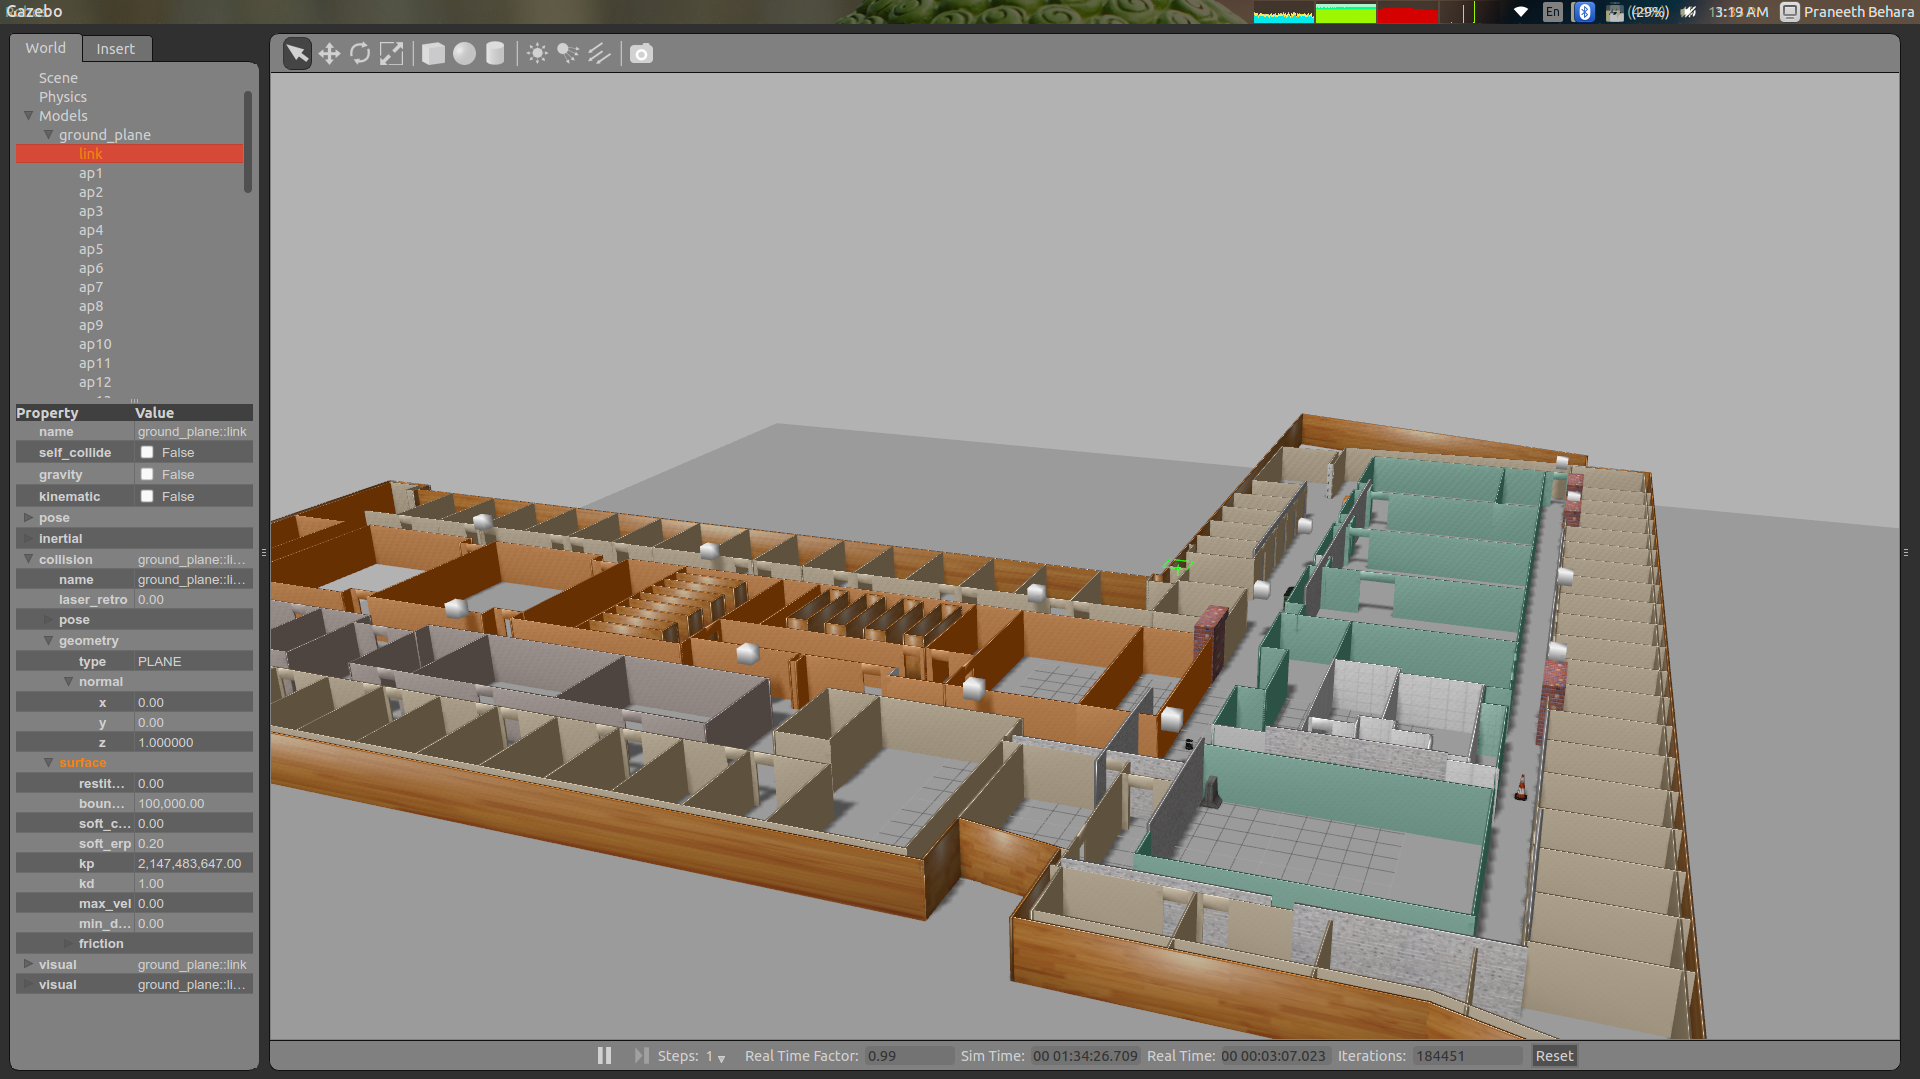
\includegraphics[width=0.49\textwidth]{images/davis3g2.png}
		\label{subfig:b}
		\caption{}
	\end{subfigure}
\caption{Shows a 100x80m to scale simulation environment of Davis Hall, UB, created using Gazebo building editor for this work.}
\end{figure*}

% \subsubsection{SDF}

% \subsection{RTAB-Map}

\subsection{Tools and Packages used}
ROS modules and packages which were used for SLAM and navigation are described below. Also other tools which help maintain the huge code base and help visualize and debug are mentioned as well. 

\textbf{RTAB-Map}: Real-Time Appearance-Based Mapping\cite{50} is a RGB-D SLAM approach based on a global loop closure detector with real-time constraints. This package can be used to generate a 3D point clouds of the environment and$/$or to create a 2D occupancy grid map for navigation. It has a Graph SLAM approach based on a global Bayesian loop closure detector. A bag-of-words approach is used to determine how likely a new image comes from an already visited location or a new one. A new constraint to the map's graph is added when a loop closure hypothesis is accepted. A graph optimizer then minimizes the errors in the map. To limit the number of locations used for loop closure detection and graph optimization, a memory management approach with short-term and long term memories are used. RTAB-Map can be used alone with a hand-held Kinect or stereo camera for 6DoF RGB-D mapping, or a laser rangefinder for 3DoF mapping. \url{http://wiki.ros.org/rtabmap} 

\textbf{move\_base}: This package helps in moving the robot to desired positions in the map using ROS navigation stack. It uses the actionlib package to achieve the above through actions. The move\_base node links together a global and local planner to accomplish its global navigation task. \url{http://wiki.ros.org/move_base}

\textbf{RViz}: 3D visualization tool for ROS. Used to display 3D sensor data, exploration trajectories, maps and to handle user input. \url{http://wiki.ros.org/rviz} 

\textbf{Gitlab}: A version control software which stores code base, tracks any changes made and helps maintaining multiple version for switching and testing. It also allows group sharing and collaboration. \url{https://gitlab.com} % Experimental Setup

\chapter{Experiments and Results}
\lhead{\emph{Evaluation}}
This chapter presents the results of implementation of frontier based exploration using Wi-Coverage with a single robot, tested in different simulated environments. The simulation environments are created using Gazebo simulator. Later we discuss in detail, the technicalities faced while realizing the frontier based exploration in the real world and ways to solve them. 

\section{System Setup}
A Turtlebot configured with Kinect Xbox 360 and an Nvidia TK1 CPU is used in this work(see chapter 3). Gazebo simulation software was used for experimenting in different simulated environments. For visualizing the constructed map and for other debugging purposes such as visualizing identified frontiers, frontier selections, origin of occupancy grid, trajectory planned by move\_base, local and global costmaps, simulated AP locations, etc, Rviz has been used. The robot is equipped with SLAM packages and exploration strategies, signal strength models are varied through controller.py node in the ndrones ROS package. Results evaluated for Wi-Coverage are based on time taken to explore and percentage of area covered vs time. 

% \section{Frontier Exploration}
% \begin{figure}
%     \centering
%     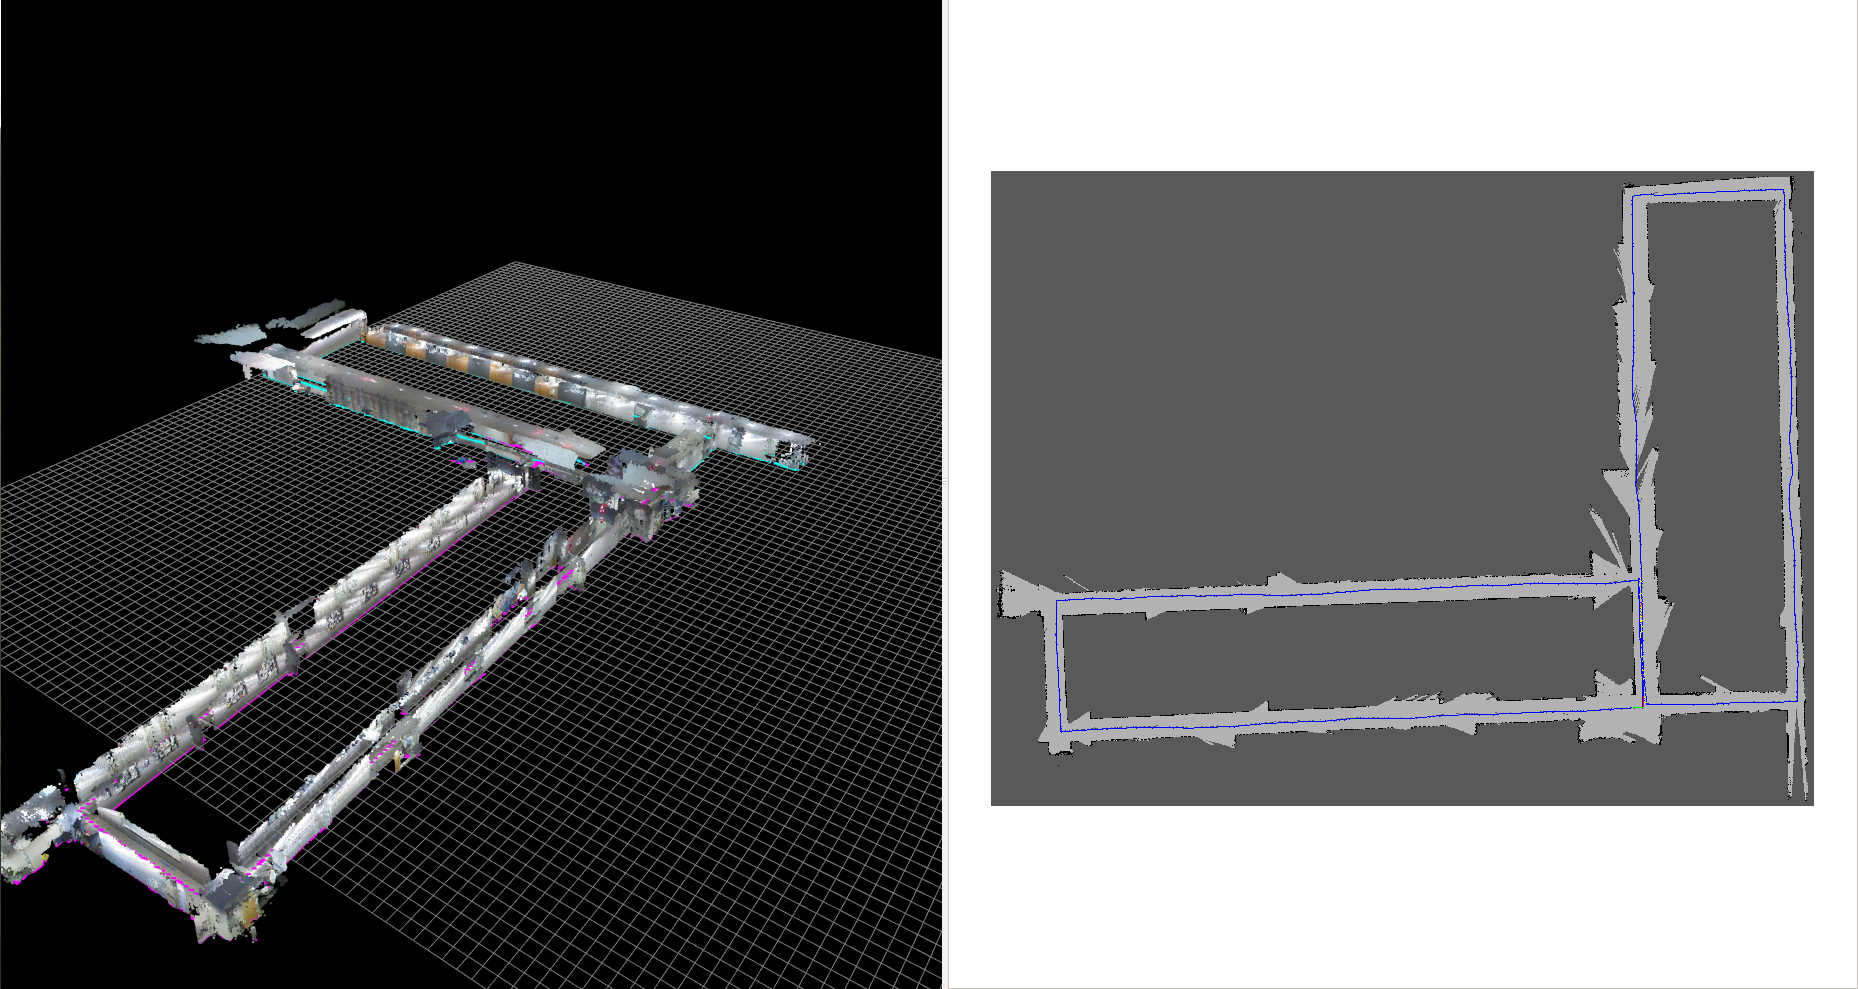
\includegraphics[width=0.75\textwidth]{images/Davis3.png}
%     \caption{Full coverage time in free space shown in Fig. xxx}
%     \label{fig:freespace}
% \end{figure}

\section{Wi-Fi}
To implement and evaluate our proposed exploration algorithm, multiple environments have been created using Gazebo simulator. Since no modules to simulate Wi-Fi APs were available we have implemented our own Wi-Fi simulation modules for the experiments. To simulate explorations in different environments using simulated Wi-Fi, we used two signal strength models, the standard ITU indoor model and a custom signal strength model from \cite{30}.

\subsection{ITU indoor Model}
\begin{figure*}[!b]
\centering
	\begin{subfigure}[b]{\textwidth}
		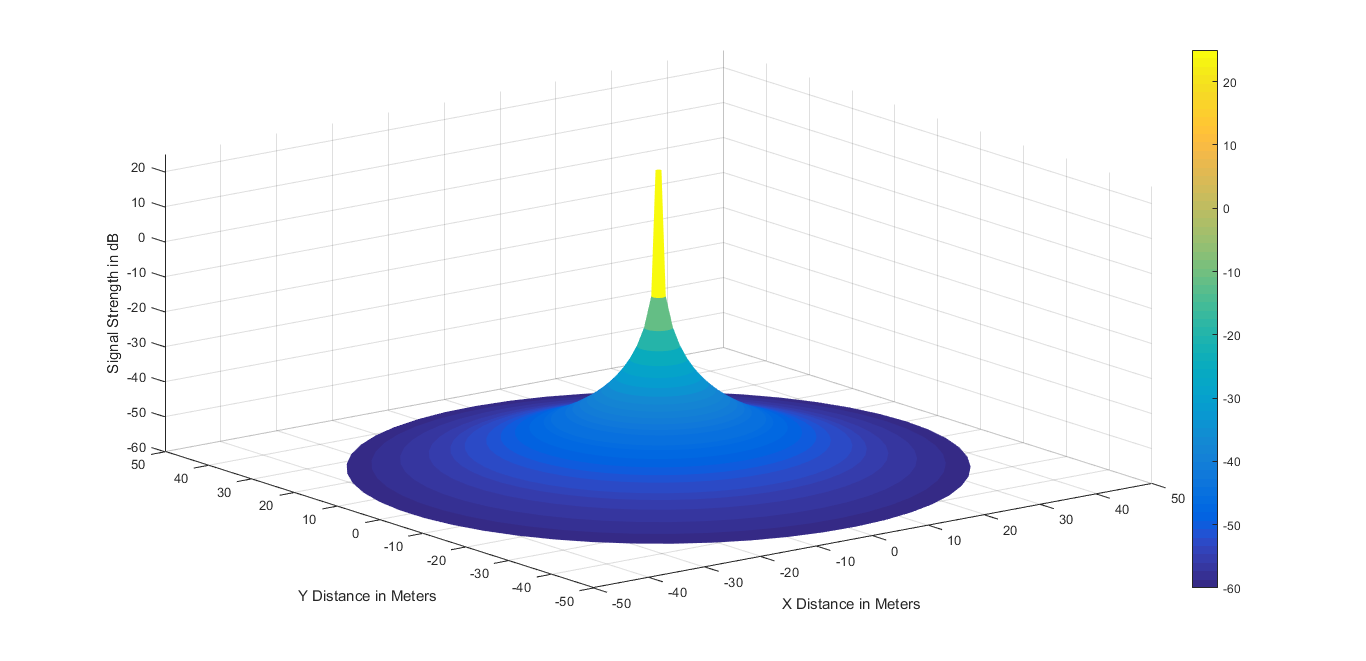
\includegraphics[width=\textwidth]{images/ITU_rm_3d.png}
		\label{subfig:a}
		\caption{}
	\end{subfigure}
    % \vfill
	\begin{subfigure}[b]{\textwidth}
		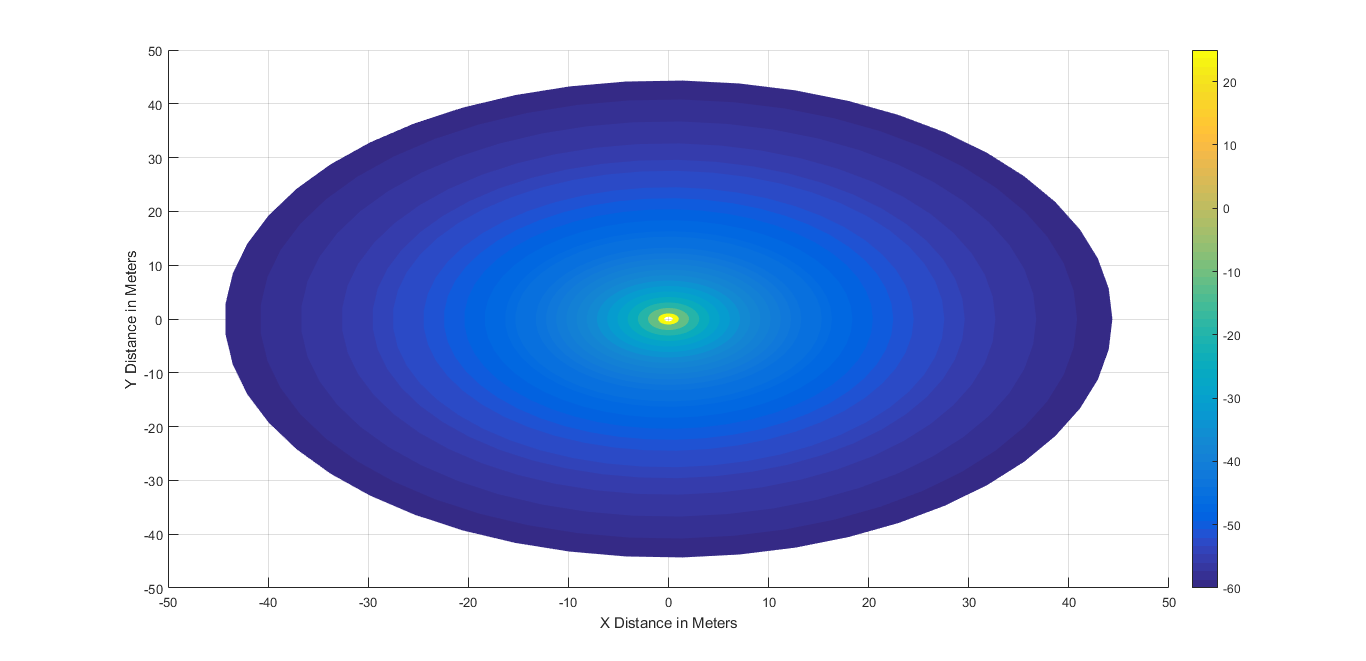
\includegraphics[width=\textwidth]{images/ITU_rm_tv.png}
		\label{subfig:b}
		\caption{}
	\end{subfigure}
\caption{Wi-Fi signal strength plot of ITU indoor model over a 100m spread}
\end{figure*}
The ITU indoor propagation model, also known as ITU model for indoor attenuation, is a radio propagation model that estimates the path loss inside a room or a closed area inside a building delimited by walls of any form. Suitable for appliances designed for indoor use, this model approximates the total path loss an indoor link may experience\cite{31}. Though this model suits best to indoor environments for appliances which use the lower microwave bands around 2.4GHz, it applies to a much wider range typically covering frequency ranges from 900MHz to 5.2GHz.\\ 
The ITU indoor path loss model is expressed as\cite{31}:
\begin{equation}
    L = 20log_{10}f + Nlog_{10}d + P_f(n) - 28
\end{equation}
where,\\
L = the total path loss (dB).\\
f = Frequency of transmission (MHz).\\
d = Distance (m).\\
N = The distance power loss coefficient.\\
n = Number of floors between the transmitter and receiver.\\
P$_f$(n) = the floor loss penetration factor.

The received power is calculated using the expression:
\begin{equation}
    P_r = P_t - (L + R_x + T_x)
\end{equation}
where,\\
P$_r$ = Power received by the receiver (dB)\\
P$_t$ = Power transmitted by AP (dB)\\
R$_x$ = Receiver sensitivity (dB)\\
T$_x$ = Transmitter gain (dB)

The values for the constants used in this work are summarized in Table 4.1. Fig 4.1 shows the pass-loss propagation model of ITU indoor model over a 100m spread. Fig 4.1 (A) shows a 3D view of the radio wave intensity vs distance and Fig 4.1 (B) shows the top view of those intensity levels. Considering the maximum power from a Wi-Fi router and a common receiver sensitivity,which is around -60dB, the signal strengths are thresholded to a high of 25dB and a low of -60dB as shown in the intensity bar plot simulating close to that of a real world. 

\begin{table}[h!]
\centering
\begin{tabular}{c c}
\hline
Variable & Value\\
\hline
f        & 2400 MHz\\
N        & 30\\
n        & 0\\
P$_f$(n) & 11\\
P$_t$    & 23\\
R$_x$    & -60\\
T$_x$    & 6\\
\hline
\end{tabular}
\caption{Table for values used in ITU attenuation model}
\label{table:1}
\end{table}

\subsection{Custom SS model}
\begin{figure*}
\centering
	\begin{subfigure}[b]{\textwidth}
		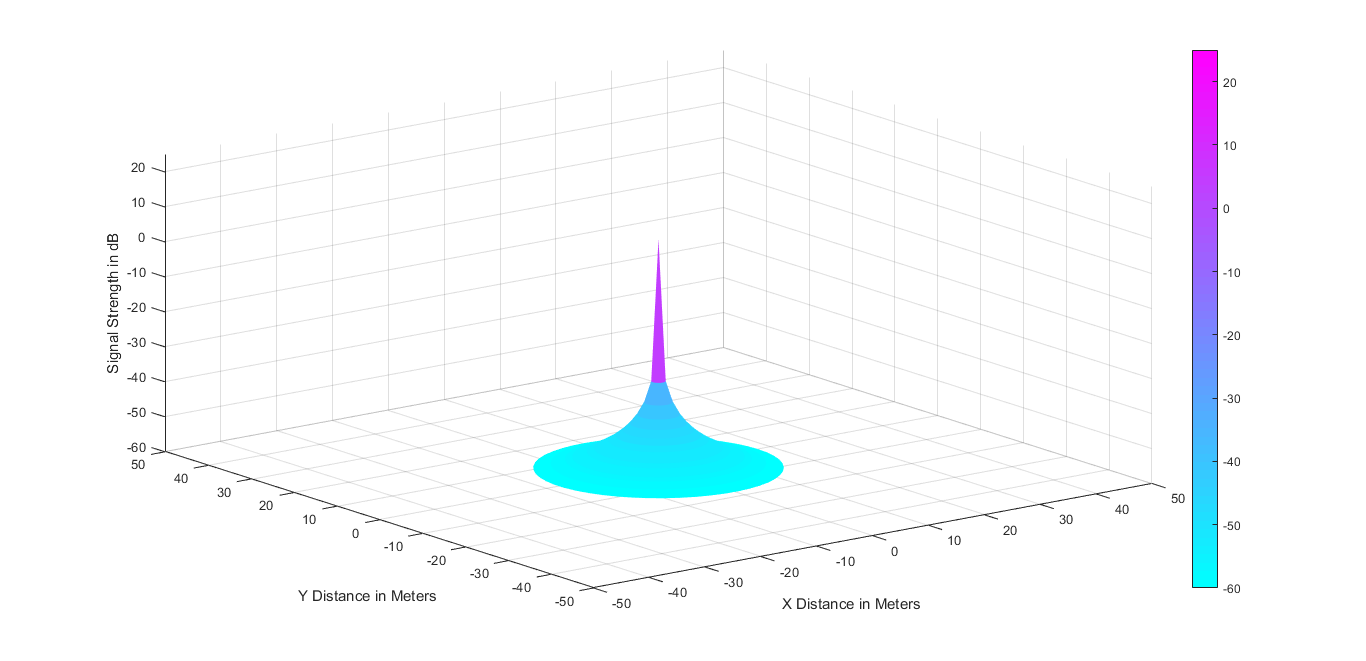
\includegraphics[width=\textwidth]{images/FAL_rm_3d.png}
		\label{subfig:a}
		\caption{}
	\end{subfigure}
    % \vfill
	\begin{subfigure}[b]{\textwidth}
		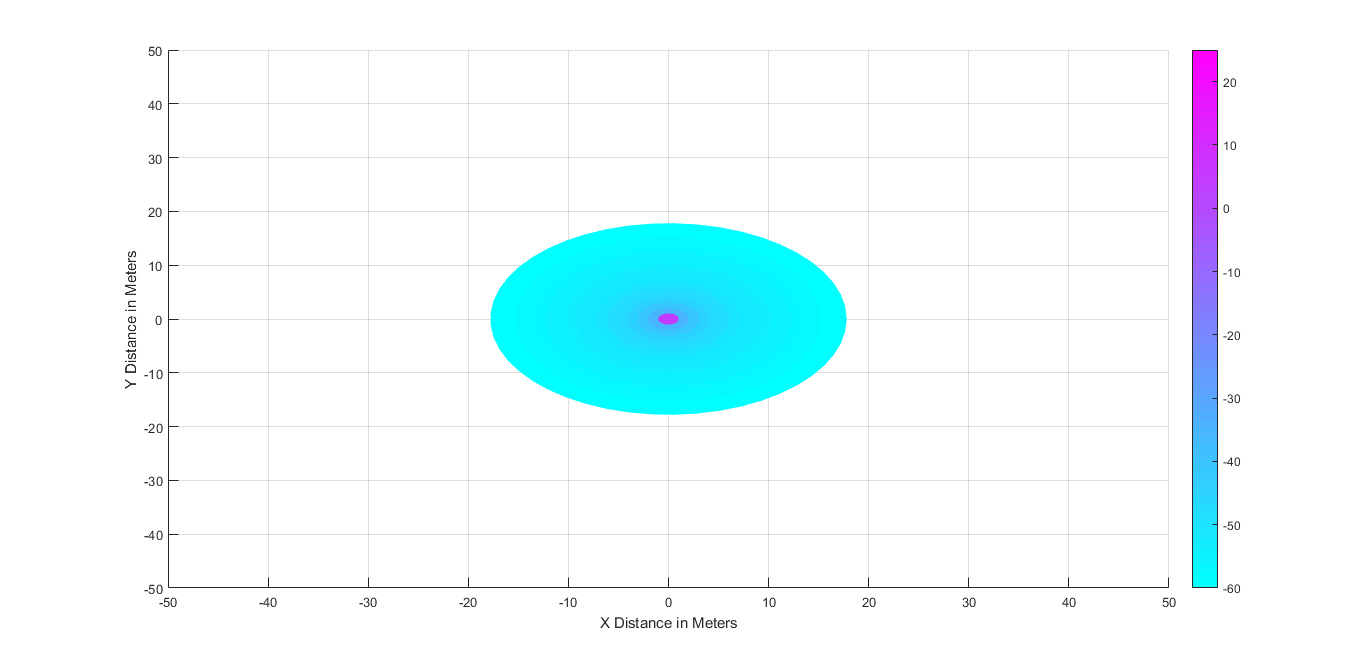
\includegraphics[width=\textwidth]{images/FAL_rm_tv.png}
		\label{subfig:b}
		\caption{}
	\end{subfigure}
\caption{Wi-Fi signal propagation model plot of CSS model over a 100m spread}
\end{figure*}
In order to extensively evaluate the performance of Wi-Coverage, we considered testing in a different radio model with lower signal intensity levels. The CSS model can be mathematically expressed as\cite{30}:
\begin{equation}
    RSS = C - 10nlog_{10}(d) + X_\sigma - 30
\end{equation}
where,\\
RSS = Power received (dB)\\
C = constant\\
n = path-loss exponent\\
X$_\sigma$ = shadow noise modeled as a Gaussian random variable with zero mean and standard deviation $\sigma_{RSS}$

\begin{table}[h!]
\centering
\begin{tabular}{c c}
\hline
Variable & Value\\
\hline
C        & -30\\
n        & 3\\
\hline
\end{tabular}
\caption{Table for values used in CSS propagation model}
\label{table:1}
\end{table}

It can be observed that the signal propagation is much weaker compared to ITU model. A regular receiver cannot sense the AP if more than 17m away.

\section{Maps}
Two maps, free space and office, are created using gazebo to evaluate Wi-Coverage using different performance metrics. Access points are placed at a height of 3m from ground level. The walls of the map are colored on purpose to provide some visual features to RTAB-Map for loop closure detection. Also both maps hold a wooden floor for the same reason and for aesthetics. All maps are unknown to robot while performing exploration and its behaviour is tested in complete autonomous mode.

\begin{figure*}[!h]
    \centering
	\begin{subfigure}[b]{\textwidth}
	    \centering
		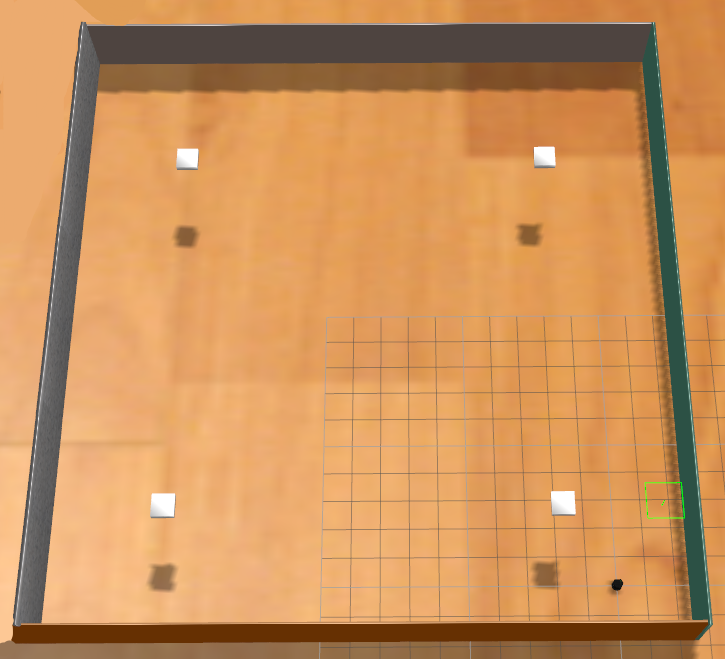
\includegraphics[width=0.5\textwidth]{images/squarespace.png}
		\label{subfig:a}
		\caption{A 30x30m free space with four Wi-Fi routers}
		\vspace{2em}
	\end{subfigure}
    % \vfill
	\begin{subfigure}[b]{\textwidth}
	    \centering
		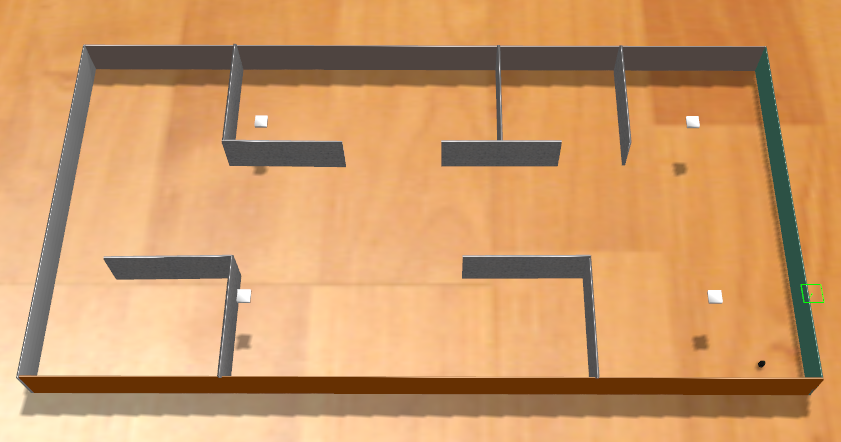
\includegraphics[width=0.75\textwidth]{images/officearea.png}
		\label{subfig:b}
		\caption{An office environment of 60x30m with four APs}
	\end{subfigure}
\caption{Maps created in Gazebo simulator with Wi-Fi APs for evaluating Wi-Coverage}
\end{figure*}

\subsection{Free Space}
Fig 4.3 (A) shows a square area of 30x30m free space powered with four simulated APs shown in white cubes.  Figs 4.4 and 4.5 shows the radio waves propagation in the free space map with four APs. The peaks represent the location of the APs. Fig 4.4 (A) is the SS vs distance plot for ITU indoor model. It is worth noting that all APs have an overlap of their signals with each other. This also implies that the robot would sense atleast one or in this case all four APs from any location in the map. Fig 4.4(B) is a top view of the previous figure. On contrary, in case of CSS model, there exist deaf spots or the places where none of the APs can be sensed. It is useful in understanding the algorithm's take on deaf spots. Also there is no overlap of signals between APs cross opposite to each other. 

\begin{figure*}[!h]
\centering
	\begin{subfigure}[b]{0.75\textwidth}
		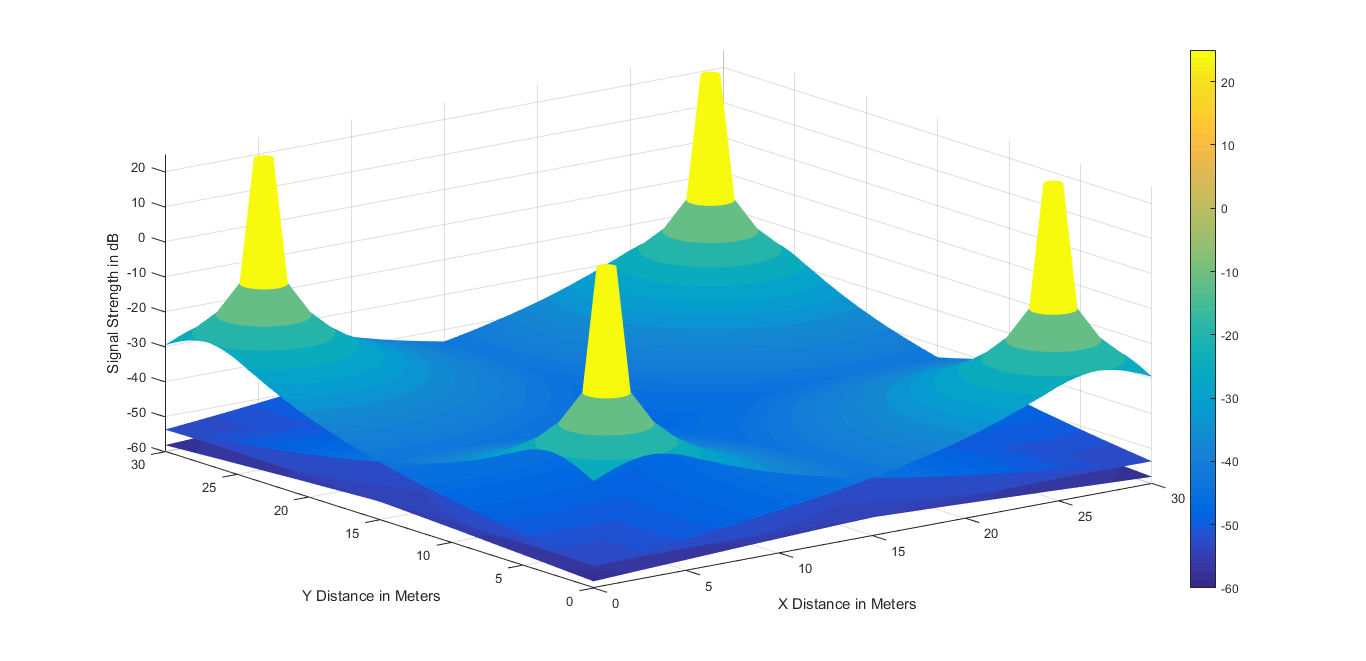
\includegraphics[width=\textwidth]{images/ITU_30x30_3d.png}
		\label{subfig:a}
		\caption{}
	\end{subfigure}
    % \vfill
	\begin{subfigure}[b]{0.75\textwidth}
		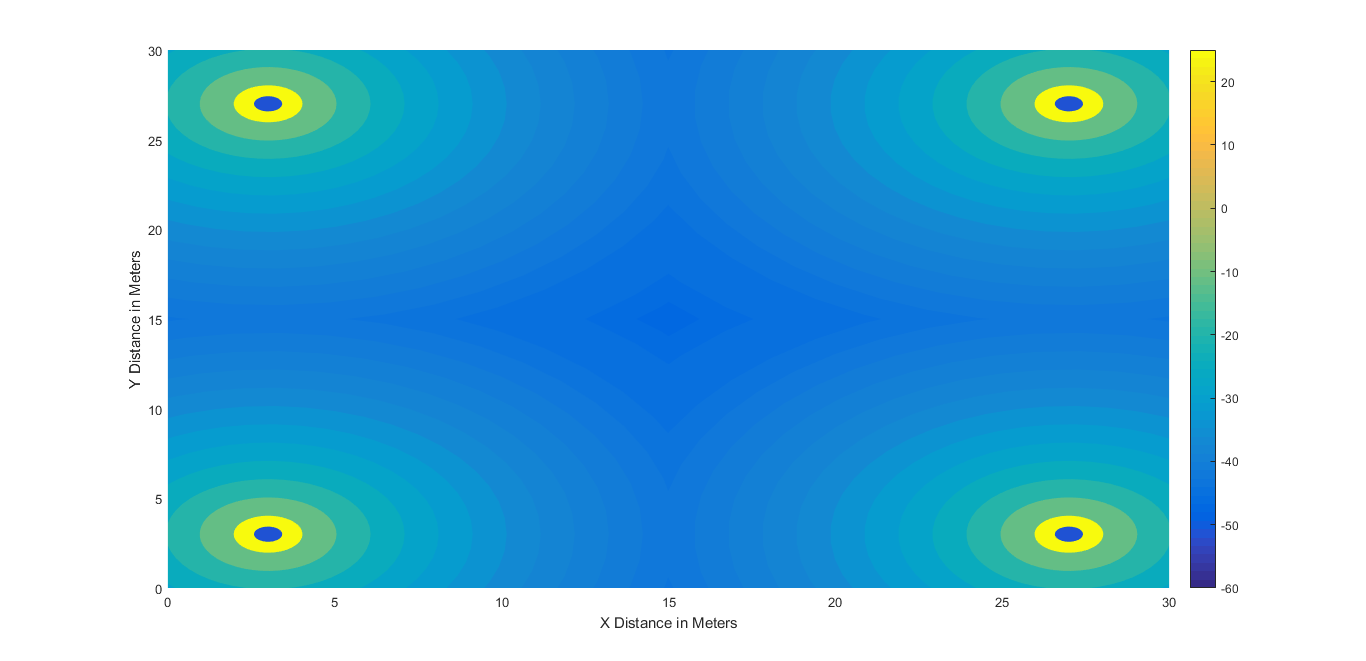
\includegraphics[width=\textwidth]{images/ITU_30x30_tv.png}
		\label{subfig:b}
		\caption{}
	\end{subfigure}
\caption{ITU propagation model in free space map with four APs. The bar chart indicates the intensity in dB}
\end{figure*}

% Fig 4.5 shows the propagation model for ITU indoor model which is much closer to reality. It has an overlap between all four APs in case of the free space map.
\begin{figure*}[!h]
\centering
	\begin{subfigure}[b]{0.75\textwidth}
		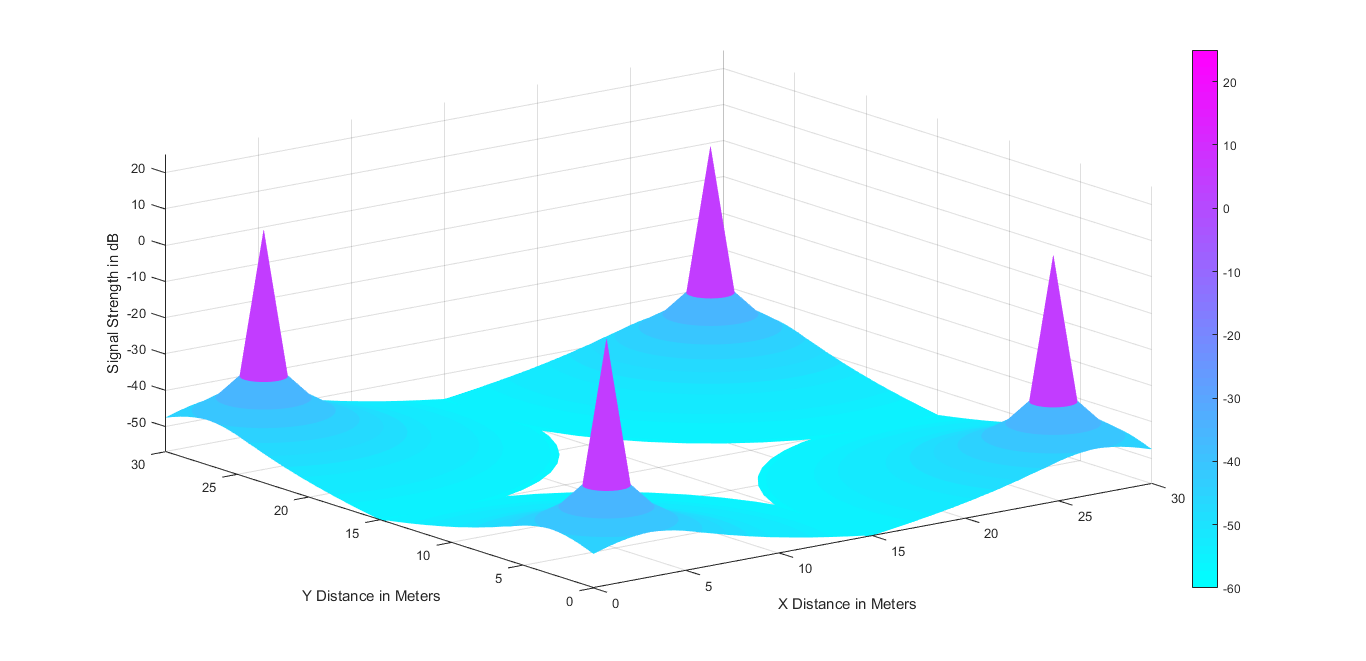
\includegraphics[width=\textwidth]{images/FAL_30x30_3d.png}
		\label{subfig:a}
		\caption{}
	\end{subfigure}
    % \vfill
	\begin{subfigure}[b]{0.75\textwidth}
		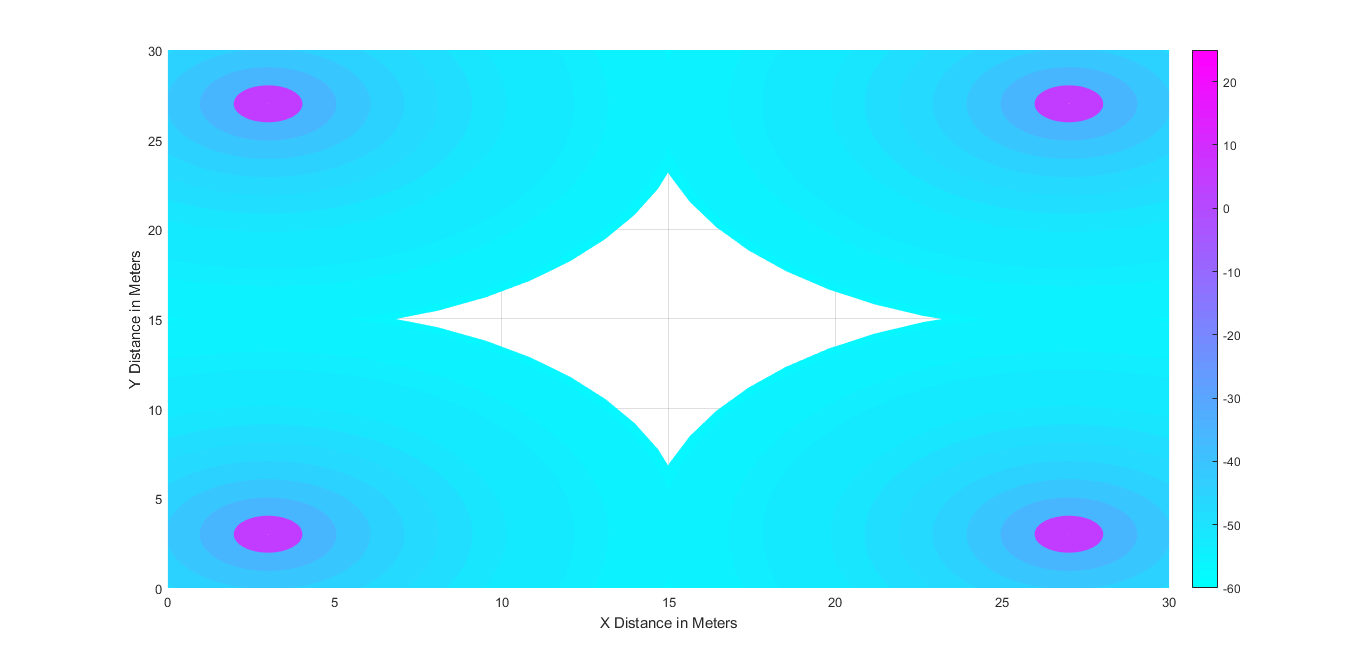
\includegraphics[width=\textwidth]{images/FAL_30x30_tv.png}
		\label{subfig:b}
		\caption{}
	\end{subfigure}
\caption{CSS propagation model in free space map with four APs. The bar chart indicates the intensity in dB}
\end{figure*}

\begin{figure}
    \centering
    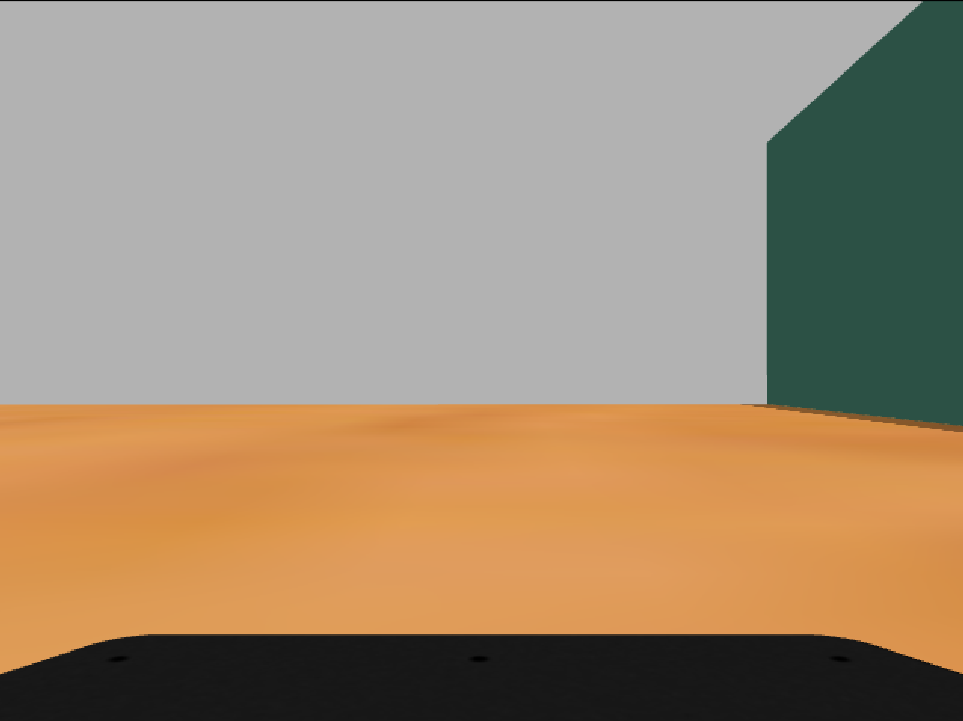
\includegraphics[width=0.5\textwidth]{images/robotview.png}
    \caption{The robots view at the start of the exploration.}
    \label{fig:freespace}
\end{figure}

\subsection{Office Space}
Fig 4.3 (B) represents a typical office space with cubicles and inlets. rectangle hall with obstacles resembling real world environment. This environment also has the same AP location configuration as that of the previous one.

\section{Coverage Results}
Simulation results are obtained for each map shown in fig 4.3 using a single robot. As mentioned before, no prior information about the environment including AP locations are provided to the robot. Maps are loaded and displayed in Gazebo for visualization and debugging purposes. Fig 4.6 represent the robots view of the environment at the start of exploration. Robot can be started at any location to achieve full coverage. Fifteen simulations are run in each environment with two different Wi-Fi signal strength models: ITU indoor model and custom signal strength(CSS) model. Results for coverage vs time contain standard deviations for each method and environment tested in. The time units used in results is real-time seconds obtained from ROS time.

\subsection{Robot Trajectories}
Robot trajectories are plotted for each method in both the SS models to present the robots systematic behaviour. All Wi-Coverage trajectories plotted are color coded. Each color represent an AP and its associated robot trajectory. Smaller points represent the frontier poses picked by the robot and lines represent the robot trajectory. The color of the line represent the robots exploration in the corresponding AP cluster. Each cluster has its own color same as that of its AP and a change in the line color implies that the robot has completely explored the current cluster and is moving to the next best cluster as per the algorithm. The bigger color dots in the graphs show that the robot has entered a different AP cluster while exploring the current cluster. Color of the dot represent the AP cluster it realizes and associates all new frontiers to that cluster (see chapter 3). Also all robots start from the origin which is at bottom right corner. The following is a legend explaining the representations involved in the trajectory plots.

\begin{figure}[!h]
    \centering
    \includegraphics[width=0.2\textwidth]{images/legend.png}
    \caption{A legend for robot trajectory plots of Wi-Coverage}
    \label{fig:freespace}
\end{figure}

\subsubsection{Free Space Robot Trajectories}

\begin{figure*}[!h]
\centering
	\begin{subfigure}[b]{\textwidth}
	    \centering
		\includegraphics[width=0.95\textwidth]{images/traj_cm_30x30.png}
		\label{subfig:a}
		\caption{CSS model}
	\end{subfigure}
    % \vfill
	\begin{subfigure}[b]{\textwidth}
	    \centering
		\includegraphics[width=0.95\textwidth]{images/30x30_itu_traj_final.png}
		\label{subfig:b}
		\caption{ITU model}
	\end{subfigure}
\caption{Robot trajectories in free space map}
\end{figure*}

This environment is created relatively simple with no obstacles which will help evaluate the free form of Wi-Coverage in performing online clustering. It also helps evaluating the robots movement when compared to other methods. Fig 4.8 and 4.9 show the plots of Darwin's trajectory in free space map using Wi-Coverage and Information gain based frontier exploration. In case of Wi-Coverage, there are always a finite set of possible trajectories which can be helpful in predicting robots next move if necessary. The trajectories shown is one such possibility which we recorded while experimenting. They keep varying based on the sensor's accuracy and varying signal strengths especially in case of CSS model due to a shadow noise added in the propagation model. 

\par Fig 4.8 (A) shows a trajectory in CSS model with four APs. The robot starts with cluster AP1 and identifies two frontiers cells in cluster AP2. It can be noticed that the robot chose the last red pose (6.3, 4.2) which completely explores the cluster AP1 and moves ahead to cluster AP2. Later it moves to cluster AP3 as an unexplored frontier opened previously by the robot while exploring cluster AP1. The robot then completely explores cluster AP3 and finally its successful exploration comes to an end after exhausting all frontiers of cluster AP4. Similarly in the ITU model due to a bigger overlap, the robot has opened frontiers from all the unexplored clusters and sorts them. This information is later used to select the next best cluster based on the information gains of the cluster's unexplored frontiers. Robot trajectory for frontier exploration using optimal information gain policy is shown in Fig 4.9. It can be noticed that the breadths and depths of the search are not well defined and is highly unpredictable.

\begin{figure}[!b]
    \centering
    \includegraphics[width=0.75\textwidth]{images/infosquare.png}
    \caption{Robot trajectory in free space map using Information gain based exploration}
    \label{fig:info}
\end{figure}

\subsubsection{Office Space Robot Trajectories}
Office map is a relatively complex environment that simulates real world obstacles like walls and inlets like cubicles. This map is spread across an area of 60x30m and powered by four APs capable of simulating two radio signal propagation models for testing. Robot trajectories for both SS model configurations are shown in the Fig 4.10. Wi-Coverage helps achieve a systematic exploration. From the trajectory graphs it can clearly observed that, the robot finishes exploring the cubicles under an AP completely and later moves to the other cubicles thereby completely covering the entire space in a systematic, breadth and depth defined like search. On the other hand information gain method made the robot move along the hallway and later cover the left over cubical spaces increasing the robot trial and hence coverage time. This can particularly be a disadvantage when exploring offices with long hallways. The difference in propagation model has not effected Wi-Coverage much, since in deaf spots the robot continuous to explore based on information gain until it senses an AP which triggers Wi-Coverage.    

\begin{figure*}[!h]
\centering
	\begin{subfigure}[b]{\textwidth}
	    \centering
		\includegraphics[width=0.95\textwidth]{images/trajitu.png}
		\label{subfig:a}
		\caption{CSS model}
		\vspace{2em}
	\end{subfigure}
    % \vfill
	\begin{subfigure}[b]{\textwidth}
	    \centering
		\includegraphics[width=0.95\textwidth]{images/trajcss.png}
		\label{subfig:b}
		\caption{ITU model}
	\end{subfigure}
\caption{Robot trajectories in the office space}
\end{figure*}

\begin{figure}[!h]
    \centering
    \includegraphics[width=0.75\textwidth]{images/trajig1.png}
    \caption{Robot trajectory in office space using information gain based exploration.}
    \label{fig:info}
\end{figure}

\subsection{Coverage Area vs Time}
Both the methods compared, explore completely any given space since both methods use frontier exploration. The only difference is in the method of allocating frontiers. Since exploration is a time sensitive problem, coverage time is an important metric to be considered for evaluation. 

\subsubsection{Free Space}

Fig 4.11 (A) plots the time taken to completely cover the environment in free space map with two propagation models: ITU model and CSS model. Wi-Coverage is compared to optimal information gain policy in both models. Minimum, Maximum and average times taken to explore completely are shown in the plot. The numbers on the top of the bars show the average time for that method. Fig 4.11(B) shows a plot of percentage coverage area vs time. Time taken to cover every quarter percentage area of total space is plotted. Information gain based exploration has the best average time of 821.32 secs followed closely by Wi-Coverage strategy with also a 100\% coverage in an average time of 875.86 and 904.32 secs in CSS and ITU models respectively. 

\begin{figure*}[!h]
\centering
	\begin{subfigure}[b]{0.75\textwidth}
		\includegraphics[width=\textwidth]{images/full_ct.png}
		\label{subfig:a}
		\caption{Free Space}
	\end{subfigure}
    % \vfill
	\begin{subfigure}[b]{0.75\textwidth}
		\includegraphics[width=\textwidth]{images/freespace.png}
		\label{subfig:b}
		\caption{Office Space}
	\end{subfigure}
\caption{Percentage Coverage Area vs time in free space}
\end{figure*}

\subsubsection{Office Space}
The coverage results for office environment are plotted in Fig 4.12. Fig 4.11(A) shows the plot of full coverage time for both methods in different SS models. Information gain based exploration explored the complete space in an average time of 1874.56 secs. Wi-Coverage in CSS model achieves this in an average time of 1892.48 secs which is closely followed by Wi-Coverage in ITU indoor model completing the entire space in 1902.12 secs. The coverage results of Wi-Coverage are pretty comparable to the information gain approach. Fig 4.12(B) shows the percentage area covered vs time. It is clear from the results that Wi-Coverage trails very close to the gold standard of frontier exploration. Fig 4.12 plots the percentage covered area with time for Information gain based exploration and Wi-Coverage in ITU indoor model. This graph explains that information gain based exploration has a quicker percentage of area covered at the beginning since it mostly explores the hallway first. But at the end, the coverage time increases due to longer trails in order to reach unexplored patches. On contrary, Wi-Coverage  almost had a linear relationship between percent area covered and time except at some places where we observe a dip. These minor dips occur due to the rejection of most optimal frontier in order to visit already queued frontier of the same cluster which is the basis of Wi-Coverage: to first exhaust the frontiers of current cluster before moving to the next. But this is almost compensated at the end of the exploration since the robot has to make smaller trails to finish the remaining unexplored space.  

\begin{figure*}[!h]
\centering
	\begin{subfigure}[b]{0.75\textwidth}
		\includegraphics[width=\textwidth]{images/bargoffice.png}
		\label{subfig:a}
		\caption{Free Space}
	\end{subfigure}
    % \vfill
	\begin{subfigure}[b]{0.75\textwidth}
		\includegraphics[width=\textwidth]{images/60x30office.png}
		\label{subfig:b}
		\caption{Office Space}
	\end{subfigure}
\caption{Percentage Coverage Area vs time in office space}
\end{figure*}

\section{Issues}
The primary reason is the exploration strategy, which decides, which sensor the robot adorns. As discussed in the previous chapters, there are a number of approaches for autonomous robot exploration. In this work we used RGB-D data from a vision sensor which is a Kinect Xbox 360 and a visual slam package RTAB-Map to perform autonomous exploration using a frontier based approach. This setup used is common in all the experiments and the following issues and solutions are particular to the sensor and packages(See Chapter 3) used in this work, unless explicitly specified.  

\subsection{Glass and reflective surfaces}

\begin{figure}
    \centering
    \includegraphics[width=0.75\textwidth]{images/Glass_ppt.png}    
    \caption{Sensor scan representing failed detection of a transparent(Glass) surface}
    \label{fig:my_label}
\end{figure}

Walls and windows made of glass can be found in almost any urban setting such as airports, malls, offices and even some homes. 
Light sensors like stereo cameras or lidars are incapable of detecting such transparent and reflective surfaces. This is a common problem faced in any exploration or mapping application. Figure 4.14 above shows an experiment (snapshot from Rviz) conducted in Davis Hall, University at Buffalo. The robot performs a sensor sweep to identify frontiers and assumes an empty space beyond the glass doors which was later accounted for containing frontiers and the robot bumps into the glass. Similarly, when a reflective surface is confronted by such sensors, the point cloud would contain the reflection thereby effecting the algorithm's judgment.

\lhead{\emph{Issues}}
\textbf{Solution}:
A traditional and probably the only simple solution is to use a sonar. The sonar is swept across the environment along with the vision sensor and the evidence grid is updated by filtering such specular reflections and transparent obstacles such as glass by limiting the range to that of sonar. The disadvantage in this approach is the addition of a new equipment to the robot making it expensive and bulky.

\subsection{Sensor uncertainty}
When frontiers detected are false or redundant, explored space is re-explored increasing the coverage time  and thereby reducing the efficiency. This happens when the sensor model estimate is erroneous in a portion of the map explored and calculations are performed on it without pre-processing or filtering. For example, when a sensor sweep is performed and the sensor is uncertain about the occupancy of a grid cell, corresponding evidence grid is erroneous thereby effecting all the consequent stages in the algorithm. Fig. 4.15 below shows such a scenario. The sensor model was unsure in classifying some grid cells to empty or occupied hence resulting in an unknown grid cell which in fact was an empty cell. Later with this occupancy grid, the next best point was formulated to be this false unknown cell lying in between empty cells which were already mapped and added to the point cloud. This redundant move increased the full coverage time of the exploration making it inefficient. 

\begin{figure}
    \centering
    \includegraphics[width=0.75\textwidth]{images/falsefrontier.png}
    \caption{A false frontier detected in an explored empty space}
    \label{fig:my_label}
\end{figure}

\textbf{Solutions}: 
This issue can be overcomed using two approaches,
\begin{itemize}
    \item \textbf{Custom resolution} : One of the approach to overcome redundant frontiers is to increase the resolution of the occupancy grid generated. In general, this is a parameter in the mapping package which can be tweaked. If not, a custom occupancy grid(bigger than the original) is to be generated with a policy that determines the final occupancy of the cell based on the threshold count of type of cells in the original grid. For example, if the grid has 98\% of empty cells and 2\% of unknown cells, it is safe to consider the occupancy of the cell in the new resolution grid as empty which eliminates spurious frontiers in already mapped areas.
    \item \textbf{Post processing} : Another approach would be to post process the frontiers identified and threshold them such that only valid frontiers are queued. Again, the thresholding can be performed based on the neighbouring grid cells irrespective of the resolution of the current occupancy grid.  
\end{itemize}

\subsection{Dynamic environments}
Obstacles moving in the environment could effect identifying frontiers turning them out as false ones. Fig 4.16 represent an exploration trial wherein at one of the sensor sweeps a door was opened and tiny points from the sensor are added to the point cloud. Later the door was closed and as expected the next best goal was inside the room since the information gain around the point was large. The robot performs a failed attempt to move to the goal position since the path was blocked and rejects the frontier after it reaches the maximum times of attempts. 

\textbf{Solution}:
Most implementations follow the traditional approach of having a maximum number of attempts the robot can have in reaching its next best position in the environment. Having reached the maximum number of tries, the respective frontier is deemed inaccessible and the robot attempts to reach the next best frontier in the queue. Though this practice works well, the exploration time would drastically increase in a clustered environment especially with decent sized robots whose footprint matters such as of a Turtlebot. As mentioned above, post processing the frontiers can help eliminate such futile attempts to reach frontiers which creep into the point cloud due to the dynamicity in the environment saving the time for exploration. 
\begin{figure*}
    \begin{subfigure}[b]{0.498\textwidth}
		\includegraphics[width=\textwidth, height=0.6\textwidth]{images/maprate.png}
		\label{subfig:a}
		\caption{}
	\end{subfigure}
	\begin{subfigure}[b]{0.498\textwidth}
		\includegraphics[width=\textwidth, height=0.6\textwidth]{images/map2.png}
		\label{subfig:b}
		\caption{}
	\end{subfigure}
\caption{(A) Image shows a dynamic environment: Door behind the bot being opened and later closed. (B) Shows the corresponding point cloud after a sensor scan containing the creeped-in points when the door was open. The green cube shows the next best point to which the bot was supposed to plan its path but could not since the door was closed.}
\end{figure*}

\subsection{False loop closures}
The ability to understand if a place has already been visited or not is the crux of loop closing. Once the robot identifies that its current immediate environment has been previously visited, it stitches the global map at this point. It is quite common that if the robot senses a similar environment else where, the map is stitched at the wrong place making the mapped environment clumsy and incorrect, This is referred to as detecting a false loop closure. False loop closures are one of the major concerns in SLAM community and quite a lot of research is being carried out \cite{22}\cite{23}. 
Fig 4.17 below demonstrates a scenario of such false loop closure detected by RTAB-Map at default loop closure settings. 

\begin{figure*}
    \begin{subfigure}[b]{0.497\textwidth}
		\includegraphics[width=\textwidth, height=0.7\textwidth]{images/loop1.png}
		\label{subfig:a}
		\caption{RTAB-Map processing RGB features from the sensor data.}
		\vspace{2em}
	\end{subfigure}
	\begin{subfigure}[b]{0.497\textwidth}
		\includegraphics[width=\textwidth, height=0.7\textwidth]{images/loop2.png}
		\label{subfig:b}
		\caption{Turtlebot moving to the next best frontier point indicated as green cube.}
		\vspace{2em}
	\end{subfigure}
% 	\hfill
	\begin{subfigure}[b]{0.497\textwidth}
		\includegraphics[width=\textwidth, height=0.7\textwidth]{images/loop3.png}
		\label{subfig:c}
		\caption{RTAB-Map detects similarities in features with that of in the previous scene.}
	\end{subfigure}
    % \vfill
	\begin{subfigure}[b]{0.497\textwidth}
		\includegraphics[width=\textwidth, height=0.7\textwidth]{images/loop4.png}
		\label{subfig:d}
		\caption{Performs a false loop closure. Turtlebot's pose is changed and map is erroneously updated.}
	\end{subfigure}
\caption{Demonstrates a false loop closure using RTAB-Map}
\end{figure*}

\clearpage
\textbf{Solution}:
Visual SLAM algorithms such as RTAB-Map use memory schemes to eliminate false loop closures\cite{22} which work well in real time but does have edge cases which can fail the algorithm. For instance, if the robot has to map a very long corridor, a possibility exist that the feature has been moved to long term memory making the robot incapable to close the loop when the start point is revisited.

\subsection{Sensor shortcomings}
Kinect’s impact has extended far beyond the gaming industry\cite{24}. With its wide availability and low cost, many researchers and practitioners in computer science, electronic engineering, and robotics are leveraging the sensing technology to develop creative new ways to interact with machines and to perform other tasks, such as mapping an unknown environment. Technical specifications of this device has been listed in chapter 3. But it comes with its own shortcomings as well. Sensor like Kinect is incapable of detecting thin obstacles such as chair legs etc especially when the object falls below 0.8m range. Fig 4.18 shows a failed test run where the Turtlebot bumped into a chair and handicapped itself.

\begin{figure*}[!h]
\centering
	\includegraphics[width=0.75\textwidth]{images/chairleg.png}
\caption{Image shows a Turtlebot getting stuck after bumping into a chair}
\end{figure*}

\subsection{Obstacles}
Due to occupancy grid resolution from RTAB-Map being extremely high, i.e 0.05m, the obstacles detected rise sharp from the empty. The potential problem occurs when the next best position selected is close to the obstacle. In such case, the robot often hits the obstacles in order to move to an unreachable position relative to its foot print. 

\textbf{Solution}: Inflating the obstacles and filtering the potential unreachable frontiers can eliminate the problem. Fig 4.19(A) shows the obstacles identified from the occupancy grid. Gaussian smoothing has been applied to the obstacles and the original obstacle depths are superimposed onto the smoothed obstacles as shown in Fig 4.19(B). Frontiers lying in the gaussian zone are eliminated preventing the risk of robot hitting the obstacle or getting stuck near it.

\begin{figure*}
    \begin{subfigure}[b]{0.498\textwidth}
		\includegraphics[width=\textwidth, height=\textwidth]{images/inflation.png}
		\label{subfig:a}
		\caption{}
	\end{subfigure}
	\begin{subfigure}[b]{0.498\textwidth}
		\includegraphics[width=\textwidth, height=\textwidth]{images/inflated_obs.png}
		\label{subfig:b}
		\caption{}
	\end{subfigure}
\caption{Inflation of obstacles}
\end{figure*}




























 % Experiment 1

\chapter{Conclusions}
\lhead{\emph{Conclusions}}
This chapter presents the highlights of the material covered in the preceding chapters, going through the main contributions and discuses some avenues of future work.

\section{Summary of contributions}
We began with the observation that Wi-Fi information can be used in assisting autonomous robots in exploration. Chapter 2 presented a summary of related technical aspects which laid the foundation for the following chapters. It introduced autonomous robots and their prerequisites to become autonomous explorers. Then we looked into various forms of mapping techniques to understand the environment in a robots perspective. Coverage problem, being one of the motivations for this work is discussed in detail. A summary of existing exploration methods and coverage strategies for both single and multi robot scenarios were then presented.
\par Chapter 3 which is the core of this work introduces a novel approach to handle coverage in indoor spaces. Wi-Coverage, the coverage strategy which integrates Wi-Fi sensing with frontier based exploration to systematically and completely cover any given environment has been discussed. This chapter also presented the robot Darwin used in this work. In particular the hardware and software construction and components used were outlined.
\par Chapter 4 highlights the experiments and results conducted and evaluated using Wi-Coverage. Frontier exploration using optimal gain approach is a gold standard in autonomous exploration. We compare Wi-Coverage with it in various scenarios and environments. First, we created two different maps using Gazebo to simulate real world scenarios for simulations. Second, in order to simulate Wi-Fi, we created our own nodes in ROS. We also gave APs the ability to simulate two different signal strength models which helps in extensive testing of Wi-Coverage. Since exploration is time sensitive, we choose full coverage time in different signal propagation environments and percentage area covered vs time as our metrics. In order to truly appreciate the novelty of Wi-Coverage, robot trajectories are plotted and described. 
\par We show that our approach uses a freely available sensor and uses it to assist exploration without adding any cost or bulk to the robot. Finally, we prove that Wi-Coverage not only has a similar coverage time as the gold standard but also systematically covers the space allowing some predictability of the robots movement. It clearly shows that using Wi-Coverage the robot can overcome the limitations of its primary sensors and can understand its environment, plan its motion in a much greater sense. Also, we satisfy all the requirements for an algorithm to be reliable and realizable in the real world.
\par Lastly, we present some engineering issues faced in this work in order to make frontier exploration realizable in the real world using a Turtlebot, a stereo camera and ROS. We also provide solutions, both traditional and custom created for this work.

\section{Future work}
There is plenty of scope for future improvements and improvisations to the work presented in this thesis. Some fulfillment's and interesting directions include:

\textbf{Real time experiments} : The results obtained for frontier based exploration approach using a stereo camera and required packages from ROS have been extensively tested on a physical robot and in a real environment. But for the Wi-Coverage results are obtained using simulated environments in gazebo simulator. Though the simulations are close enough to reality, these have ideal conditions which suggests a future enhancement of testing the novel algorithm in real environments and with multiple physical robots. Also this algorithm can be tested using various sensors and results can be analyzed. 

\textbf{Exploration in 3D} : Wi-Coverage has been designed and implemented on a derived 2D occupancy grid. The robot senses the signal strength from ground level and it is assumed to be constant along the \textit{z} axis wrt the robot, i.e the altitude. An enhancement to this approach is to use 3D occupancy grid where each cell is now a voxel and area is now volume. Identifying frontiers are much challenging and computationally less expensive techniques can be developed. Clustering in layers of a 3D space using Wi-Fi signal strength and giving robots(ex aerial UAVs or robots which walk the stairs) a sense of altitude to explore and map large structures such as airports will be our future work. 

\textbf{Localize Wi-Fi routers} : Many applications such as positioning Wi-Fi routers for best coverage in a given space, indoor localization, etc requires the position estimate of the Wi-Fi routers. As Wi-Coverage involves listening to APs for signal strengths, the database collected while exploring can be used to localize them. Methods like \cite{29}\cite{30} can be used for AP localization and thereby use the routers as landmarks to improve the robot localization. 

\section{Concluding Remark}
First, this thesis has presented a way of implementing frontier based exploration with a mobile robot using just a vision sensor and extensively discussed the engineering problems faced. Second, we developed a novel online coverage solution for mobile robots in operating spaces using Wi-Fi as an additional sensor. We hope that our work, and specifically the conjecture of using Wi-Fi as an additional sensor will be useful in the development of fully autonomous exploration systems and for improving various other applications. % Experiment 2

% \input{Chapters/Chapter6} % Results and Discussion

%\input{Chapters/Chapter7} % Conclusion

%% ----------------------------------------------------------------
% Now begin the Appendices, including them as separate files

\addtocontents{toc}{\vspace{2em}} % Add a gap in the Contents, for aesthetics

\appendix % Cue to tell LaTeX that the following 'chapters' are Appendices

% \chapter{An Appendix}

Lorem ipsum dolor sit amet, consectetur adipiscing elit. Vivamus at pulvinar nisi. Phasellus hendrerit, diam placerat interdum iaculis, mauris justo cursus risus, in viverra purus eros at ligula. Ut metus justo, consequat a tristique posuere, laoreet nec nibh. Etiam et scelerisque mauris. Phasellus vel massa magna. Ut non neque id tortor pharetra bibendum vitae sit amet nisi. Duis nec quam quam, sed euismod justo. Pellentesque eu tellus vitae ante tempus malesuada. Nunc accumsan, quam in congue consequat, lectus lectus dapibus erat, id aliquet urna neque at massa. Nulla facilisi. Morbi ullamcorper eleifend posuere. Donec libero leo, faucibus nec bibendum at, mattis et urna. Proin consectetur, nunc ut imperdiet lobortis, magna neque tincidunt lectus, id iaculis nisi justo id nibh. Pellentesque vel sem in erat vulputate faucibus molestie ut lorem.

Quisque tristique urna in lorem laoreet at laoreet quam congue. Donec dolor turpis, blandit non imperdiet aliquet, blandit et felis. In lorem nisi, pretium sit amet vestibulum sed, tempus et sem. Proin non ante turpis. Nulla imperdiet fringilla convallis. Vivamus vel bibendum nisl. Pellentesque justo lectus, molestie vel luctus sed, lobortis in libero. Nulla facilisi. Aliquam erat volutpat. Suspendisse vitae nunc nunc. Sed aliquet est suscipit sapien rhoncus non adipiscing nibh consequat. Aliquam metus urna, faucibus eu vulputate non, luctus eu justo.

Donec urna leo, vulputate vitae porta eu, vehicula blandit libero. Phasellus eget massa et leo condimentum mollis. Nullam molestie, justo at pellentesque vulputate, sapien velit ornare diam, nec gravida lacus augue non diam. Integer mattis lacus id libero ultrices sit amet mollis neque molestie. Integer ut leo eget mi volutpat congue. Vivamus sodales, turpis id venenatis placerat, tellus purus adipiscing magna, eu aliquam nibh dolor id nibh. Pellentesque habitant morbi tristique senectus et netus et malesuada fames ac turpis egestas. Sed cursus convallis quam nec vehicula. Sed vulputate neque eget odio fringilla ac sodales urna feugiat.

Phasellus nisi quam, volutpat non ullamcorper eget, congue fringilla leo. Cras et erat et nibh placerat commodo id ornare est. Nulla facilisi. Aenean pulvinar scelerisque eros eget interdum. Nunc pulvinar magna ut felis varius in hendrerit dolor accumsan. Nunc pellentesque magna quis magna bibendum non laoreet erat tincidunt. Nulla facilisi.

Duis eget massa sem, gravida interdum ipsum. Nulla nunc nisl, hendrerit sit amet commodo vel, varius id tellus. Lorem ipsum dolor sit amet, consectetur adipiscing elit. Nunc ac dolor est. Suspendisse ultrices tincidunt metus eget accumsan. Nullam facilisis, justo vitae convallis sollicitudin, eros augue malesuada metus, nec sagittis diam nibh ut sapien. Duis blandit lectus vitae lorem aliquam nec euismod nisi volutpat. Vestibulum ornare dictum tortor, at faucibus justo tempor non. Nulla facilisi. Cras non massa nunc, eget euismod purus. Nunc metus ipsum, euismod a consectetur vel, hendrerit nec nunc.	% Appendix Title

%\input{Appendices/AppendixB} % Appendix Title

%\input{Appendices/AppendixC} % Appendix Title

\addtocontents{toc}{\vspace{2em}}  % Add a gap in the Contents, for aesthetics
\backmatter

%% ----------------------------------------------------------------
\label{Bibliography}
\lhead{\emph{Bibliography}}  % Change the left side page header to "Bibliography"
\bibliographystyle{unsrtnat}  % Use the "unsrtnat" BibTeX style for formatting the Bibliography
\bibliography{Bibliography}  % The references (bibliography) information are stored in the file named "Bibliography.bib"

\end{document}  % The End
%% ----------------------------------------------------------------